% -*- Mode:TeX -*-

%% IMPORTANT: The official thesis specifications are available at:
%%            http://libraries.mit.edu/archives/thesis-specs/
%%
%%            Please verify your thesis' formatting and copyright
%%            assignment before submission.  If you notice any
%%            discrepancies between these templates and the 
%%            MIT Libraries' specs, please let us know
%%            by e-mailing thesis@mit.edu

%% The documentclass options along with the pagestyle can be used to generate
%% a technical report, a draft copy, or a regular thesis.  You may need to
%% re-specify the pagestyle after you \include  cover.tex.  For more
%% information, see the first few lines of mitthesis.cls. 

%\documentclass[12pt,vi,twoside]{mitthesis}
%%
%%  If you want your thesis copyright to you instead of MIT, use the
%%  ``vi'' option, as above.
%%
%\documentclass[12pt,twoside,leftblank]{mitthesis}
%%
%% If you want blank pages before new chapters to be labelled ``This
%% Page Intentionally Left Blank'', use the ``leftblank'' option, as
%% above. 

\documentclass[12pt,vi]{mitthesis}
\usepackage[paper=a4paper,top=2.2cm, bottom=1.5cm, outer=1cm, inner=2.1cm]{geometry}% http://ctan.org/pkg/geometry
\usepackage{lgrind}
%% These have been added at the request of the MIT Libraries, because
%% some PDF conversions mess up the ligatures.  -LB, 1/22/2014
\usepackage{cmap}
\usepackage[T1]{fontenc}
%% Package "lmodern" added by user request see ServiceNow INC0396734 -OT, 4/29/2020
\usepackage{lmodern}
\pagestyle{plain}
\usepackage{tikz}
\usepackage{pdfoverlay}
\usepackage[ddmmyyyy]{datetime}
\renewcommand{\dateseparator}{.}
\usepackage{float}
\usepackage{xurl}
\usepackage{hyperref}
\usepackage{amsmath}
\usepackage{subcaption}
\usepackage{booktabs}
\usepackage{listings}
\usepackage{pifont}% http://ctan.org/pkg/pifont
\newcommand{\cmark}{\ding{51}}%
\newcommand{\xmark}{\ding{55}}%
\usetikzlibrary{positioning}

\def\abstract{
\vspace{5cm}
\begin{center}%
{\bfseries \abstractname\vspace{-.5em}}%
\end{center}
\quotation
}
\def\endabstract{\par
\endquotation
}

% Default fixed font does not support bold face
\DeclareFixedFont{\ttb}{T1}{txtt}{bx}{n}{12} % for bold
\DeclareFixedFont{\ttm}{T1}{txtt}{m}{n}{12}  % for normal

% Custom colors
\usepackage{color}
\definecolor{deepblue}{rgb}{0,0,0.5}
\definecolor{deepred}{rgb}{0.6,0,0}
\definecolor{deepgreen}{rgb}{0,0.5,0}

% Python style for highlighting
\newcommand\pythonstyle{\lstset{
language=Python,
basicstyle=\ttm,
otherkeywords={self},             % Add keywords here
keywordstyle=\ttb\color{deepblue},
emph={MyClass,__init__, modify, predict, explain_instance, append, concatenate, DataFrame, groupby, sort_values, as_list, , to_numeric, predict_proba, array, LimeTabularExplainer, fit, GaussianHMM, get_stationary_distribution, DecisionTreeClassifier},          % Custom highlighting
emphstyle=\ttb\color{deepred},    % Custom highlighting style
stringstyle=\color{deepgreen},
frame=tb,                         % Any extra options here
numbers = left,
breaklines,
xleftmargin = 15pt,
showstringspaces=false            % 
}}


% Python environment
\lstnewenvironment{python}[1][]
{
\pythonstyle
\lstset{#1}
}
{}

\begin{document}

% \newgeometry{top=6cm,bottom=2.2cm,right=0.83cm,left=3.47cm}
\pagestyle{empty}
% \pdfoverlaySetPDF{cover.pdf}
\begin{center}

% {\large \textbf{PRACA DYPLOMOWA MAGISTERSKA}}
% \vspace{6cm}

{\large \textbf{RAPPORT DE STAGE}}
\vspace{8cm}

{\fontsize{18}{18}\selectfont \textbf{Hybrid neural networks for anomaly detection in~cyber-physical systems}}
\end{center}
\normalsize

% \vspace{6cm}
% \textbf{Wydział Fizyki Technicznej, Informatyki i Matematyki Stosowanej \\
% Promotor:} dr hab. inż. Aneta Poniszewska-Marańda\\
% \textbf{Dyplomant:} inż. Ramzi Hadrich\\
% \textbf{Nr albumu:} 227488\\
% \textbf{Kierunek:} Informatyka\\
% \textbf{Specjalność:} Computer Science \& Information Technology\\
% \begin{center}
%     Łódź, \today r.
% \end{center}

\vspace{8cm}
\noindent Ramzi HADRICH \\
\textbf{Entreprise:} LORIA\\
\textbf{Tuteur Entreprise:} Abdelkader LAHMADI\\
\textbf{Tuteur ENSEM:} Radu RANTA\\
\textbf{Filière:} ISN\\
\begin{center}
    \today
\end{center}

% First copy: start a new page, and save the page number.
\cleardoublepage
\newgeometry{top=2.2cm, bottom=1.5cm, outer=1cm, inner=2.1cm}
% Uncomment the next line if you do NOT want a page number on your
% abstract and acknowledgments pages.
\begin{abstract}
Nowadays cyber-physical systems are widely used in different application domains. In parallel, machine learning algorithms are used widely to detect the anomalies in the behaviour of these systems. However, this detection is limited to two states: normal behaviour and faulty functioning. This work aims to extend this detection to differentiate between attacks and normal faults. In first place, a power system is described as an example to work on. Then, various machine learning algorithms are evaluated on the given datasets, and this using two machine learning toolkits - scikit-learn and Weka. Later, various tools for feature analysis are presented and an algorithm to find the features that contributed the most into the false predictions is described. Finally, three solutions to the initial problem are presented and evaluated - one solution uses the features found in the previous step and modifies their values, the second shrinks the samples from the dataset to have only the previously mentioned features and evaluates the distance between those samples and the third solution uses the Hidden Markov Model. The test have shown that the best performing solution was the second, even if the gain in accuracy is not very significant.  
\end{abstract}

\newpage
\renewcommand{\abstractname}{Résumé}
\begin{abstract}
De nos jours, les systèmes cyber-physiques sont largement utilisés dans différents domaines d'application. Parallèlement, les algorithmes d'apprentissage automatique sont largement utilisés pour détecter les anomalies dans le comportement de ces systèmes. Toutefois, cette détection se limite à deux états : un comportement normal et un fonctionnement défectueux. Ce travail vise à étendre cette détection afin de différencier les attaques des défauts liés au fonctionnement normal. En premier lieu, un système d'alimentation est décrit comme un exemple sur lequel on va travailler. Puis, divers algorithmes d'apprentissage machine sont évalués sur les ensembles de données donnés, et ce à l'aide de deux boîtes à outils d'apprentissage machine - scikit-learn et Weka. Ensuite, différents outils d'analyse des caractéristiques sont présentés et un algorithme permettant de trouver les caractéristiques qui ont le plus contribué aux fausses prédictions est décrit. Enfin, trois solutions au problème initial sont présentées et évaluées - une solution qui utilise les caractéristiques trouvées dans l'étape précédente et qui modifie leurs valeurs, la deuxième qui réduit les échantillons de l'ensemble de données pour n'avoir que les caractéristiques mentionnées précédemment et qui évalue la distance entre ces échantillons et la troisième solution qui utilise le modèle de Markov caché. Les tests ont montré que la solution la plus performante était la seconde, même si le gain de précision n'est pas très significatif.  
\end{abstract}


% Additional copy: start a new page, and reset the page number.  This way,
% the second copy of the abstract is not counted as separate pages.
% Uncomment the next 6 lines if you need two copies of the abstract
% page.
% \setcounter{page}{\thesavepage}
% \begin{abstractpage}
% \input{abstract}
% \end{abstractpage}

\cleardoublepage

\section*{Preface and acknowledgements}

This thesis was written in the framework of my 5-month internship at LORIA (Laboratoire Lorrain de Recherche en Informatique et ses Applications) in Nancy, France, within my Erasmus+ exchange, from September 2019 to July 2020, at Ecole Nationale Supérieure d'Electricité et de Mécanique (ENSEM), which is a part of University of Lorraine.

Despite COVID-19 pandemic, it was possible to continue and finish the work from home. Mr Abdelkader Lahmadi and Mr Jérome François were there for me during the whole period of the internship. I wanted to say thank you to both of them, for the continuous help, which made this thesis a reality. I wanted also to thank Mr Lahmadi for proposing me this research project.

I am also thankful to the international office team at my home university as well as to my supervisor Mrs Aneta Poniszewska-Marańda for making this Erasmus+ exchange possible.

Finally, I wanted to thank also my family and friends for the support during the writing process of this thesis.
%%%%%%%%%%%%%%%%%%%%%%%%%%%%%%%%%%%%%%%%%%%%%%%%%%%%%%%%%%%%%%%%%%%%%%
% -*-latex-*-


\pagestyle{plain}

\tableofcontents
\newpage
\listoffigures
\newpage
\listoftables

\chapter{Introduction} \label{chap:intro}

Cyber Physical Systems (CPS) are nowadays widely used in different application domains, such as smart-homes, smart-cities, hospitals, etc... They are mainly composed of two entities: a cyber part consisting in a computing and networking component, and a physical part consisting in different controllers and sensors. The existence of a connected cyber part implies its susceptibility to multiple cyber threats. The malfunctioning of these systems, due to a cyber threat, can cause severe impacts on the real life and the safety of the community, for example a blackout or water contamination. That is why many algorithms have been designed for the security monitoring of those systems, in particular the anomaly and attack detection.

Nowadays, machine and deep learning algorithms are used to detect those anomalies and intrusions. But, in majority, they rely only on the cyber part of the systems and on the data describing their behaviour, ignoring their physical models. The idea behind this work is to employ a hybrid machine learning algorithm, in particular neural networks, to detect anomalies and attacks in CPS considering its physical model.

\section{Physic guided machine learning in literature}

As mentioned before, the aim of the work is to fuse the black-box and theory-based models together to get better predictions. However this is not the first time such a fusion is examined. In the literature various approaches of the fusion of neural networks with theory-based models were presented. Those approaches can be divided into two types given what aspect of the algorithm they're changing: those that modify in first place the input to take into consideration the physical constraints, and those that modify the structure of the neural network.

-->here comes some more explanations--<

% In the following chapters, it was decided to start with a less complex algorithms than neuron networks, so that the interpretation would be a lot simpler, in order to generalise the findings on the neural networks in further chapters. That is why the next chapter will talk about comparing some basic machine learning methods.

\section{Case study}
In order to focus on the implementation of the hybrid machine learning algorithm, a CPS, with ready to use datasets, was chosen from a list provided in \cite{morris_industrial_nodate}: the \textbf{power system} \cite{adhikari_power_2014}, which network diagram was represented on figure \ref{fig:cps_rep}. The system is composed of two power generators who are alimenting the whole system. Intelligent Electronic Devices (IEDs) R1 to R4 and the breakers BR1 to BR4 can be found connected directly to those generators. Each IED switches its corresponding breaker when a fault is detected, valid or fake. The communication between the IEDs and the Substation Switch is done wirelessly. On the other hand the Substation Switch is connected with the Primary Domain Controller (PDC) and the Control Room.

\begin{figure}[H]
    \centering
    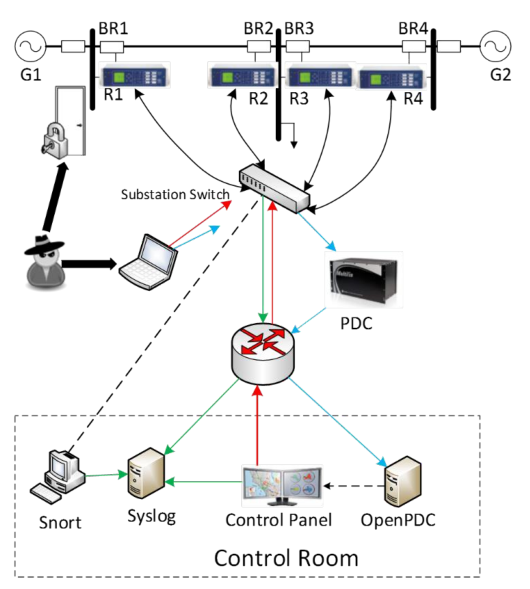
\includegraphics[width=100mm]{images/cps_rep.png}
    \caption[Power system network diagram]{Power system network diagram \cite{adhikari_power_2014}}
    \label{fig:cps_rep}
\end{figure}

The operation of this power system can be described following 6 main scenarios:
\begin{itemize}
    \item normal behaviour, 
    \item short-circuit,
    \item line maintenance,
    \item remotely opening the breakers (attack),
    \item disruption of fault protection system (attack),
    \item fault imitation (attack).
\end{itemize} 
Each of those scenarios can be divided into several sub-scenarios concerning different entities of the system or/and the failure range. Every scenario was labelled with a number between 1 and 41. In this way \textbf{37 scenarios} are obtained, divided and numbered as follows:
\begin{itemize}
    \item 1 no events scenario, its number it is 41,
    \item 8 natural fault scenarios, its number ranges are 1-6 (short-circuit) and 13-14 (line maintenance),
    \item 28 attack scenarios, its number ranges are 7-12 (fault imitation), 15-20 (remotely opening the breakers), 20-30 and 35-40 (disruption of fault protection system).
\end{itemize}
The reason for dropping the numbers between 31 and 34 in the naming process of scenarios is not known.

The datasets provided in \cite{morris_industrial_nodate} represent \textbf{78377 events}, in which one of those scenarios was reproduced in the system. They have been grouped by scenario into 3 datasets: binary (attack or normal operation), three-class (attack, normal fault and no events) and multiclass (differentiating all 37 scenarios). Each of these 3 datasets is composed of 15 .arff or .csv files comporting in average 141 events for each of 37 scenarios. The exact number of events per file for each scheme is illustrated on figure \ref{fig:scen_distro_37}. For the 3 class dataset \textbf{55663 attack}, \textbf{18309 natural fault} and \textbf{4405 normal operation} events were found. The distribution of these schemes throughout the files is shown on figure~\ref{fig:scen_distro_file}. 

\begin{figure}[H]
    \centering
    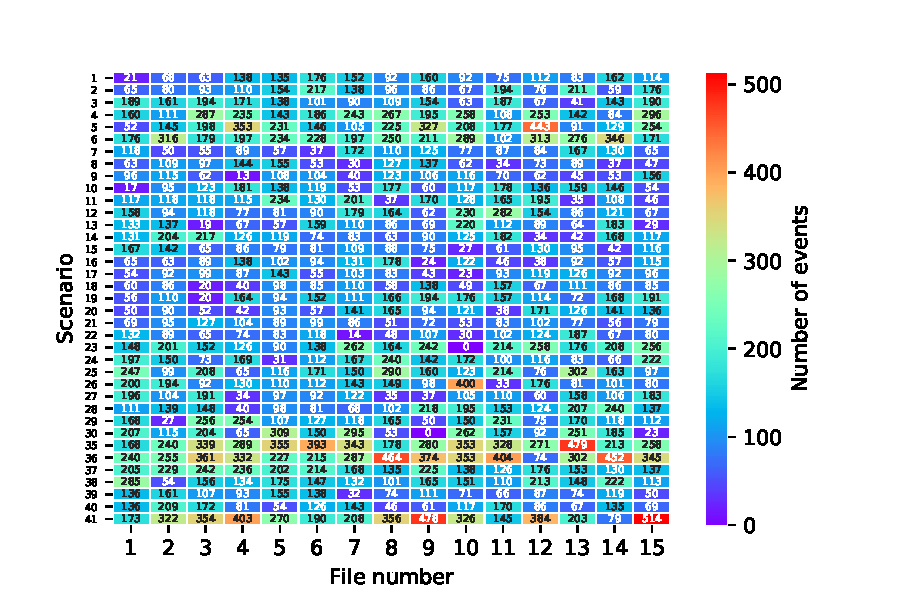
\includegraphics[]{images/distr_allscen.pdf}
    \caption{Scenarios distribution throughout all 15 files} \label{fig:scen_distro_37}
\end{figure}

\begin{figure}[H]
    \centering
    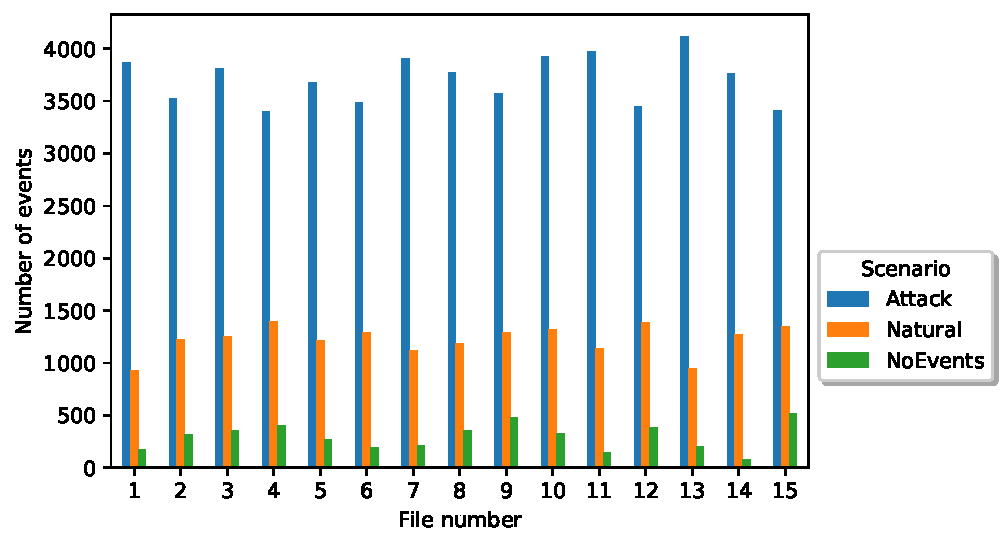
\includegraphics[]{images/distr_3classes.pdf}
    \caption{Scenarios distribution throughout the 3-class dataset files}
    \label{fig:scen_distro_file}
\end{figure}

Figure \ref{fig:scen_distro_file} shows also this distribution for the binary datasets, it is sufficient to add the number of natural (orange) and normal operation (green) events.

The scenarios are not equally distributed in the case of the 37 schemes dataset, it is especially shown by the standard deviation of 61, which is an important value compared to some scenarios counting less than 100 events. On the other hand, in the case of 3-class scenarios, the distribution is even more not equal compared to the 37 schemes dataset. The \textbf{mean standard deviation among all files is equal to 1767}, which is an enormous result given that some scenarios count only around 100 events.

Each of previously mentioned events is described by \textbf{128 features}: 116 provided by four phasor measurement units\footnote{Phasor measurement units measure the electrical waves on an electricity grid} (each one provides 29 types of measurements) and 12 other features are reserved for control panel logs, snort alerts, relay logs of 4 phasors. The mentioned 116 features, each has a label formed by \textbf{concatenation} of the \textbf{source phasor reference} (it can be R1, R2, R3, R4) and the \textbf{measurement name}, as provided in table \ref{tab:pmu_mes}. For example R4-PM5:I stands for phase B current phase magnitude measured by R4.
%give exemple - preciser plus les features 
%expliquer les features plus
%figure pour explication de phase, magnitude

\begin{table}[H]
    \centering
    \caption[Phasor measurements]{Phasor measurements \cite{adhikari_power_2014}} \label{tab:pmu_mes}
    \begin{tabular}{lr}
        \toprule
        Feature&Description \\
        \midrule
        PA1:VH – PA3:VH&Phase A-C Voltage Phase Angle \\
        PM1:V – PM3:V&Phase A-C Voltage Phase Magnitude \\
        PA4:IH – PA6:IH&Phase A-C Current Phase Angle \\
        PM4:I – PM6:I&Phase A-C Current Phase Magnitude \\
        PA7:VH – PA9:VH&Pos.–Neg.– Zero Voltage Phase Angle \\
        PM7:V – PM9:V&Pos.–Neg.–Zero Voltage Phase Magnitude \\
        PA10:VH - PA12:VH&Pos.–Neg.–Zero Current Phase Angle \\
        PM10:V - PM12:V&Pos.–Neg.–Zero Current Phase Magnitude \\
        F&Frequency for relays \\
        DF&Frequency Delta (dF/dt) for relays \\
        PA:Z&Appearance Impedance for relays \\
        PA:ZH&Appearance Impedance Angle for relays \\
        S&Status Flag for relays \\
        \bottomrule
    \end{tabular}
\end{table} 

Those datasets have been used in several works related to CPS cyber-attack classification, one of which is \cite{borges_hink_machine_2014-1}, where the author try to find the most accurate algorithm to predict the status of the power system. The following chapter shows an attempt to partially reproduce the results obtained by them.

\section{Case study}
In order to focus on the implementation of the hybrid machine learning algorithm, a CPS, with ready to use datasets, was chosen from a list provided in \cite{morris_industrial_nodate}: the \textbf{power system} \cite{adhikari_power_2014}, which network diagram was represented on figure \ref{fig:cps_rep}. The system is composed of two power generators who are alimenting the whole system. Intelligent Electronic Devices (IEDs) R1 to R4 and the breakers BR1 to BR4 can be found connected directly to those generators. Each IED switches its corresponding breaker when a fault is detected, valid or fake. The communication between the IEDs and the Substation Switch is done wirelessly. On the other hand the Substation Switch is connected with the Primary Domain Controller (PDC) and the Control Room.

\begin{figure}[H]
    \centering
    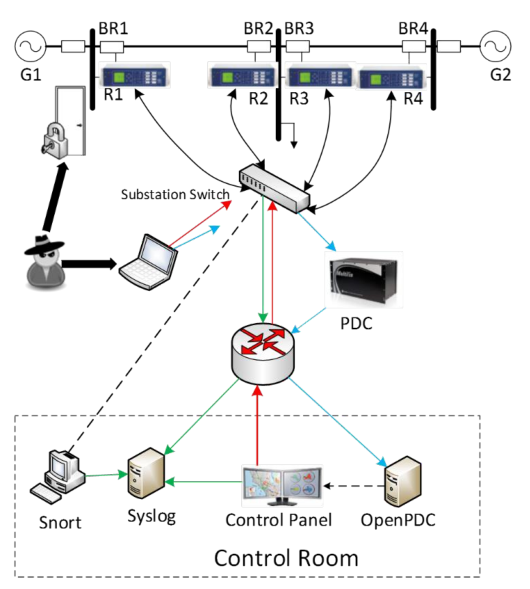
\includegraphics[width=100mm]{images/cps_rep.png}
    \caption[Power system network diagram]{Power system network diagram \cite{adhikari_power_2014}}
    \label{fig:cps_rep}
\end{figure}

The operation of this power system can be described following 6 main scenarios:
\begin{itemize}
    \item normal behaviour, 
    \item short-circuit,
    \item line maintenance,
    \item remotely opening the breakers (attack),
    \item disruption of fault protection system (attack),
    \item fault imitation (attack).
\end{itemize} 
Each of those scenarios can be divided into several sub-scenarios concerning different entities of the system or/and the failure range. Every scenario was labelled with a number between 1 and 41. In this way \textbf{37 scenarios} are obtained, divided and numbered as follows:
\begin{itemize}
    \item 1 no events scenario, its number it is 41,
    \item 8 natural fault scenarios, its number ranges are 1-6 (short-circuit) and 13-14 (line maintenance),
    \item 28 attack scenarios, its number ranges are 7-12 (fault imitation), 15-20 (remotely opening the breakers), 20-30 and 35-40 (disruption of fault protection system).
\end{itemize}
The reason for dropping the numbers between 31 and 34 in the naming process of scenarios is not known.

The datasets provided in \cite{morris_industrial_nodate} represent \textbf{78377 events}, in which one of those scenarios was reproduced in the system. They have been grouped by scenario into 3 datasets: binary (attack or normal operation), three-class (attack, normal fault and no events) and multiclass (differentiating all 37 scenarios). Each of these 3 datasets is composed of 15 .arff or .csv files comporting in average 141 events for each of 37 scenarios. The exact number of events per file for each scheme is illustrated on figure \ref{fig:scen_distro_37}. For the 3 class dataset \textbf{55663 attack}, \textbf{18309 natural fault} and \textbf{4405 normal operation} events were found. The distribution of these schemes throughout the files is shown on figure~\ref{fig:scen_distro_file}. 

\begin{figure}[H]
    \centering
    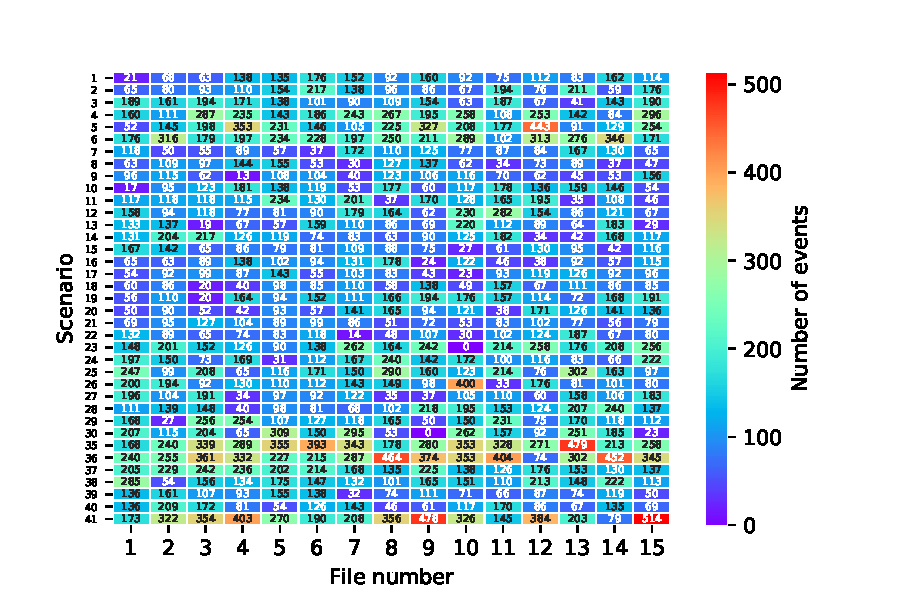
\includegraphics[]{images/distr_allscen.pdf}
    \caption{Scenarios distribution throughout all 15 files} \label{fig:scen_distro_37}
\end{figure}

\begin{figure}[H]
    \centering
    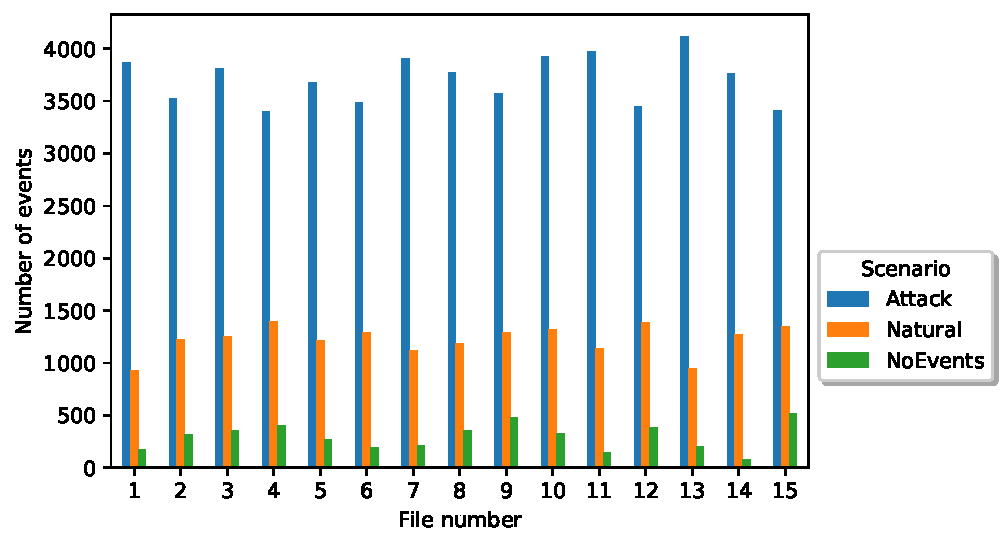
\includegraphics[]{images/distr_3classes.pdf}
    \caption{Scenarios distribution throughout the 3-class dataset files}
    \label{fig:scen_distro_file}
\end{figure}

Figure \ref{fig:scen_distro_file} shows also this distribution for the binary datasets, it is sufficient to add the number of natural (orange) and normal operation (green) events.

The scenarios are not equally distributed in the case of the 37 schemes dataset, it is especially shown by the standard deviation of 61, which is an important value compared to some scenarios counting less than 100 events. On the other hand, in the case of 3-class scenarios, the distribution is even more not equal compared to the 37 schemes dataset. The \textbf{mean standard deviation among all files is equal to 1767}, which is an enormous result given that some scenarios count only around 100 events.

Each of previously mentioned events is described by \textbf{128 features}: 116 provided by four phasor measurement units\footnote{Phasor measurement units measure the electrical waves on an electricity grid} (each one provides 29 types of measurements) and 12 other features are reserved for control panel logs, snort alerts, relay logs of 4 phasors. The mentioned 116 features, each has a label formed by \textbf{concatenation} of the \textbf{source phasor reference} (it can be R1, R2, R3, R4) and the \textbf{measurement name}, as provided in table \ref{tab:pmu_mes}. For example R4-PM5:I stands for phase B current phase magnitude measured by R4.
%give exemple - preciser plus les features 
%expliquer les features plus
%figure pour explication de phase, magnitude

\begin{table}[H]
    \centering
    \caption[Phasor measurements]{Phasor measurements \cite{adhikari_power_2014}} \label{tab:pmu_mes}
    \begin{tabular}{lr}
        \toprule
        Feature&Description \\
        \midrule
        PA1:VH – PA3:VH&Phase A-C Voltage Phase Angle \\
        PM1:V – PM3:V&Phase A-C Voltage Phase Magnitude \\
        PA4:IH – PA6:IH&Phase A-C Current Phase Angle \\
        PM4:I – PM6:I&Phase A-C Current Phase Magnitude \\
        PA7:VH – PA9:VH&Pos.–Neg.– Zero Voltage Phase Angle \\
        PM7:V – PM9:V&Pos.–Neg.–Zero Voltage Phase Magnitude \\
        PA10:VH - PA12:VH&Pos.–Neg.–Zero Current Phase Angle \\
        PM10:V - PM12:V&Pos.–Neg.–Zero Current Phase Magnitude \\
        F&Frequency for relays \\
        DF&Frequency Delta (dF/dt) for relays \\
        PA:Z&Appearance Impedance for relays \\
        PA:ZH&Appearance Impedance Angle for relays \\
        S&Status Flag for relays \\
        \bottomrule
    \end{tabular}
\end{table} 

Those datasets have been used in several works related to CPS cyber-attack classification, one of which is \cite{borges_hink_machine_2014-1}, where the author try to find the most accurate algorithm to predict the status of the power system. The following chapter shows an attempt to partially reproduce the results obtained by them.

\chapter{Machine learning algorithms comparison} \label{chap:methods}

%essayer d'autres noyaux pour SVM
%roc pour tous les scenariaux
%concatenate all datasets

%rappeler objectif
Before going further and analysing neural networks in order to create a hybrid machine learning algorithm for anomaly detection in the power distribution system presented in chapter \ref{chap:intro}, a deeper look at classical machine learning algorithms will be taken, in particular Random Forest, Support Vector Machine (SVM), NaïveBayes and multilayer perceptron. However this was done before in \cite{borges_hink_machine_2014-1} using the black-box model algorithms only. In their approach they used Weka \cite{witten_appendix_2017} in order to find the most performant algorithm among 7 they have chosen (OneR, NNge, Random Forest, Naïve Bayes, SVM, JRipper, Adaboost). 

This chapter shows an attempt to reproduce the results provided in \cite{borges_hink_machine_2014-1}, using two different machine learning toolkits (Weka and scikit-learn \cite{pedregosa_scikit-learn_2011}) in order to confirm the obtained results. That is why, first, these two toolkits will be presented, then the obtained results will be discussed.  

\section{Machine learning toolkits}
\subsection{Weka} \label{sec:weka_in_chap:methods}
%les parametres des algos, m par defaut
\textbf{Weka}, or more exactly \textbf{W}aikato \textbf{E}nvironment for \textbf{K}nowledge \textbf{A}nalysis, is an open source machine learning software developed at The University of Waikato in Hamilton, New Zealand and based on Java programming language. It is well known especially in academic environments and a lot of machine learning researches were conducted using it, one of them the mentioned before \cite{borges_hink_machine_2014-1}. It incorporates various machine learning tools: classifiers, regressors, visualizers, data pre-processor etc...

Weka is characterised by 3 main operating schemes. First, it can be run using a \textbf{graphical user interface} (GUI), enabling the user, even without deep knowledge in programming, to make machine learning experiments and analyse available classifiers. Second, more advanced users have the option to run all the available tools using a \textbf{command line}. Finally, Weka's tools can be \textbf{integrated directly into code in several programming languages (Java, Python, R, Spark)}, which enables even larger versatility.

\subsection{scikit-learn}
scikit-learn is an open-source machine learning \textbf{Python library} developed originally by David Cournapeau as a Google Summer of Code project and now it is maintained by a team of volunteers. It is well known in both academic and commercial environments, since it is used by many enterprises such as Spotify, Evernote, Booking.com, and research facilities like Inria or Télécom ParisTech \cite{noauthor_who_nodate}. It includes, just like Weka, various machine learning tools such as classifiers, regressors, data pre-processor etc... Its visualisation capabilities are limited, however there exist many additional Python packages for data visualisation such as YellowBrick, Eli5 and others... They will be further discussed in next chapter.

scikit-learn can be used only as an extension of Python language, what makes a bit harder for non experts to start working with it. However, since Python is an user friendly programming language and scikit-learn has a well made documentation, this toolkit is easy to use. Along with other Python packages, and especially pandas, scikit-learn is a very powerful, ergonomic and versatile solution for machine learning problems.  

It might be also interesting to mention that scikit-learn can be used within Weka after installing the appropriate add-on. This enables Weka users to use scikit-learn classifiers and regressors and run Python code just inside Weka's GUI.

\section{Used machine learning algorithms}
Before talking about the comparison of machine learning algorithms, the used classifiers are briefly described in this section in order to better understand how do they work. In parallel, values of classifiers' parameters used during all the tests are presented in tables \ref{tab:rf_param}, \ref{tab:svm_param} and \ref{tab:nb_param}, and, in majority, they represent the default values found in Weka, in order to reproduce the results from~\cite{borges_hink_machine_2014-1}.

\subsection{Random Forest} \label{sec:rf}
Random Forest, as the name indicates, is an \textbf{ensemble} of a given number of trees, and more exactly \textbf{decision trees}. This given number of trees is set using the parameter \textit{numIterations} in Weka and \textit{n\_estimators} in scikit-learn. Each of decision trees is created based on a randomly chosen set of features of the dataset. The number of features is given by the parameter \textit{numFeatures} in Weka and \textit{max\_features} in scikit-learn, which indicate the way it is calculated - in this case as the logarithm of base 2 of the number of features. 

On the other hand, decision trees represent a structure capable of determining the class of the predicted sample. It is composed of nodes connected to each other in a form of tree. Each node corresponds to a condition related to the features, for example if a particular feature is higher than a certain number. Each node, except the decision ones, has two child nodes corresponding to the answer as yes or no to the condition from from parent node. For each of two answers, particular classes are assigned, for example, given the case study in this work, yes answer can correspond to classes Attack and Natural and the answer no to class NoEvents. When running a tree on a particular sample, the nodes are followed given the answers on conditions, until arriving to the decision node. The class corresponding to this node is taken as the final output of the decision tree. The number of layers of nodes is called the depth of the tree and it is set using the parameter \textit{maxDepth} in both Weka and scikit-learn.

The choice of condition in a node is based on calculating \textbf{gini impurity} or \textbf{information gain} metric for each feature and determining, based on one of them, which feature has the biggest effect on the choice of the class. Gini impurity determines the probability of a feature being classified incorrectly when selected randomly, it is given by the equation:
\begin{equation}
    \text{Gini impurity} = 1 - \sum^n_{i=1} (p_i)^2,
\end{equation}
where n is the number of classes and $p_i$ the probability of the feature being classified for the class i. The information gain on the other hand, determines the quantity of information that the features gives about a particular class, it is calculated as:
\begin{equation}
    E(S) = \sum^n_{i=1} - p_i \log_2 p_i.
\end{equation}
Weka uses the information gain metric, while in scikit-learn it is possible to choose the metric using the parameter \textit{criterion}, which by default is set to gini impurity, which is less computationally complex.

The random forest, composed of a number of those decision trees, determines the class of a sample taking the class chosen by the biggest amount of decision trees. In both Weka and scikit-learn, this classifier comes with more, less crucial parameters, which are all listed in table~\ref{tab:rf_param}.

\begin{table}[H]
    \footnotesize
    \centering
    \caption{Random Forest classifier parameters} \label{tab:rf_param}
    \begin{subtable}[t]{.5\linewidth}
        \caption{Weka \cite{noauthor_randomforest_nodate}}
        \centering
        \begin{tabular}{lr}\toprule
            Parameter & Value \\\midrule
            bagSizePercent & 100\\
            batchSize & 100 \\
            breakTiesRandomly & False \\
            calcOutOfBag & False \\
            computeAttributeImportance & False \\
            debug & False \\
            doNotCHeckCapabilities & False \\
            maxDepth & 0 \\
            numDecimalPlaces & 2 \\
            numExecutionSlots & 1 \\
            numFeatures & 0 \\
            numIterations & 100 \\
            outputOutOfBagComplexityStatistics & False \\
            printClassifiers & False \\
            seed & 1 \\
            storeOutOfBagPredictions & False \\\bottomrule
        \end{tabular}
    \end{subtable}%
    \begin{subtable}[t]{.5\linewidth}
        \caption{scikit-learn \cite{noauthor_sklearnensemblerandomforestclassifier_nodate}}
        \centering
        \begin{tabular}{lr}\toprule
            Parameter & Value \\\midrule
            n\_estimators & 100 \\
            criterion & "gini" \\
            max\_depth & None \\
            min\_samples\_split & 2 \\
            min\_samples\_leaf & 1 \\
            min\_weight\_fraction\_leaf & 0.0 \\
            max\_features & "log2" \\
            max\_leaf\_nodes & None \\
            min\_impurity\_decrease & 0.0 \\
            min\_impurity\_split & None \\
            bootstrap & True \\
            oob\_score & False \\
            n\_jobs & None \\
            random\_state & None \\
            verbose & 0 \\
            warm\_start & False \\
            class\_weight & None \\
            ccp\_alpha & 0.0 \\
            max\_samples & None \\\bottomrule
        \end{tabular}
    \end{subtable}%
\end{table}

\subsection{SVM}

SVM, or more exactly \textbf{Support Vector Machine}, is a classifier that creates an N-dimensional space, in which all the samples from the training dataset are put, and then divided, geometrically, into regions, where each region corresponds to one class. The N dimensions of this space corresponds to all the features of the datasets and their transformations (for example a square of one of the features). Those transformations are done using a kernel function which can be set in Weka and scikit-learn using the \textit{kernelType/kernel} parameter. Three kernel types are more commonly used: linear, polynomial and radial basis function (exponent based). The default kernel in both Weka and scikit-learn is radial basis function. Each type of kernel function comes with a set a parameters itself, like the degree in the case of polynomial and all of them can be set through the parameters of both used machine learning toolkits.

In fact, the transformations do not calculate additional dimensions for every sample, but calculate the distance between points in the N-dimensional space. This distance is mathematically defined as the \textbf{dot product} of the two points. The dot product on other hand is defined of the sum of products of coordinates for every dimension. 

The division is made by determining so called \textbf{hyperplane}, which for example in a 2D features space is just a line. The points from each class that are the closest to the hyperplane are called \textbf{support vector points}, from where comes the name of this classifier \cite{yadav_support_2018} \cite{noauthor_support_2014}. 

The algorithm is running within a set number of iterations (can be set within Weka and scikit-learn) dividing the training dataset to smaller tranches using the cross-validation technique. The goal is to find the hyperplane that way so the number of misclassified samples is the smallest in that particular iteration. 

SVM in Weka and scikit-learn comes additionally with other parameters than are listed on table~\ref{tab:svm_param}.

\begin{table}[H]
    \footnotesize
    \centering
    \caption{SVM classifier parameters} \label{tab:svm_param}
    \begin{subtable}[t]{.5\linewidth}
        \caption{Weka \cite{noauthor_libsvm_nodate}}
        \centering
        \begin{tabular}{lr}\toprule
            Parameter & Value \\\midrule
            SVMType & C-SVC (classification) \\
            batchSize & 100 \\
            cacheSize & 40.0 \\
            coef0 & 0.0 \\
            cost & 1.0 \\
            debug & False \\
            degree & 3 \\
            doNotCHeckCapabilities & False \\
            doNotReplaceMissingValues & False \\
            eps & 0.001 \\
            gamma & 0.0 \\
            kernelType & radial basis function\\
            loss & 0.1 \\
            modelFile & Weka-3-8-4 \\
            normalize & False \\
            nu & 0.5 \\
            numDecimalPlaces & 2 \\
            probabilityEstimates & True \\
            seed & 1 \\
            shrinking & True \\
            weights & \\\bottomrule
        \end{tabular}
    \end{subtable}%
    \begin{subtable}[t]{.5\linewidth}
        \caption{scikit-learn \cite{noauthor_sklearnsvmsvc_nodate}}
        \centering
        \begin{tabular}{lr}\toprule
            Parameter & Value \\\midrule
            C & 1.0 \\
            kernel & "rbf" \\
            degree & 3 \\
            gamma & "scale" \\
            coef0 & 0.0 \\
            shrinking & True \\
            probability & True \\
            tol & 1e-3 \\
            cache\_size & 7000 \\
            class\_weight & None \\
            verbose & False \\
            max\_iter & 1000 \\
            decision\_function\_shape & "ovr" \\
            break\_ties & False \\
            random\_state & None \\\bottomrule
        \end{tabular}
    \end{subtable}%
\end{table}
 
\subsection{NaïveBayes}
NaïveBayes is a classifier based on the \textbf{Bayes theorem}, which states that the probability of event A, given that the event B happened is equal to the product of the probability of B given that A occurred and the probability of A, divided by the probability of B:
\begin{equation}
    P(A|B) = \frac{P(B|A)\dot P(A)}{P(B)}.
\end{equation}
While the naivety of the algorithm is due to it does not taking into consideration the eventual relations between the features.

The NaïveBayes classifier can be both \textbf{multinomial} and \textbf{gaussian}. In the multinomial case the probabilities are calculated the classical way (number of occurrences over all samples), whereas in the gaussian case, the probabilities are taken from the gaussian distribution of a given event. For both Weka and scikit-learn the gaussian case were used.

The list of all the parameters available is listed on table \ref{tab:nb_param}, however they impact on how the algorithm works is marginal. 

\begin{table}[H]
    \footnotesize
    \centering
    \caption{NaïveBayes classifier parameters} \label{tab:nb_param}
    \begin{subtable}[t]{0.5\linewidth}
        \caption{weka \cite{noauthor_naivebayes_nodate}}
        \centering
        \begin{tabular}{lr}\toprule
            Parameter & Value \\\midrule
            batchSize & 100 \\
            debug & False \\
            displayModelInOldFormat & False \\
            doNotCHeckCapabilities & False \\
            numDecimalPlaces & 2 \\
            useKernelEstimator & False \\
            useSupervisedDiscretization & False\\\bottomrule
        \end{tabular}
    \end{subtable}%
    \begin{subtable}[t]{.5\linewidth}
        \caption{scikit-learn \cite{noauthor_sklearnnaive_bayesgaussiannb_nodate}}
        \centering
        \begin{tabular}{lr}\toprule
            Parameter & Value \\\midrule
            priors & None \\
            var\_smoothing & 1e-9 \\\bottomrule
        \end{tabular}
    \end{subtable}%
\end{table}

\subsection{Multilayer perceptron}
The multilayer perceptron is a classifier inspired by the structure of the human brain. It is constituted from a set of interconnected neurons, which are divided into at least 2 layers: input layer, $n$ hidden layers and output layer. Each layer consist of a number of neurons. The input layer has always a number of neurons equal to the number of features, and the output layer has always this number equal to the number of outputs of the problem. That is why, in the analysed case the input layer has 128 neurons and the output layer only one neuron corresponding to the status of the power plant (normal behaviour, natural fault, attack). Each of the mentioned neurons has a weight. The neurons are interconnected. The output of a neuron is considered as the input for the neurons of the following layer. Those neurons of the following layer calculates the weighted sum of the inputs and passes the results through a function, called activation function. The result obtained this way is considered as the output of the given neuron and goes to the following layer. The only exception is the input layer, which input is the values of features and its neurons just copy the input to the output \cite{patel_implementing_2020} \cite{noauthor_neural_nodate} \cite{stokfiszewski_soft_nodate}.

The training process consists in updating the weights of the neurons during a predefined number of iterations called epochs. Before starting the training process the initial weights $w_i$ values for hidden and output layers should be chosen. This choice can be done empirically or randomly. Moreover, a real positive number $\eta$ called training step must be fixed. In each epoch and for each training pattern, the weights are updated following the equation:
\begin{equation}
    w_i = w_i + \eta\cdot (z^{(\mu)}-y) \cdot x_i^{(\mu)},
\end{equation}
where $z^{(\mu)}$ is the desired output for the $\mu$-th training sample, $y$ is the neuron output (weighted sum passed through the activation function), $x_i^{(\mu)}$ is the neuron's input value for the same $\mu$-th training sample and $i$ indicates the neuron index in the trained layer. After each epoch, the training samples are shuffled \cite{stokfiszewski_soft_nodate}. 

The scikit-learn implementation of multilayer perceptron classifier is limited because it does not give a full control of each hidden layer and its activation function. It integrates however the possibility to determine the number of epochs called iterations and the training step called learning rate. All available parameters available are shown in table \ref{tab:mlp_param}. The implementation of MLP exists also in Weka, but it is as well limited, for this reason the analysis of its results will not be taken into consideration.

There exists multiple python frameworks offering much more flexibility when creating neural networks like PyTorch \cite{noauthor_pytorch_nodate} or Keras framework \cite{noauthor_keras_nodate}, which were created in order to offer the possibility to create complex neural networks able to be used in large-scale applications. Even the developers of scikit-learn state on their website \cite{noauthor_neural_nodate}:

\begin{quote}
    \textit{This implementation is not intended for large-scale applications. In particular, \mbox{scikit-learn} offers no GPU support.} 
\end{quote}

The mentioned frameworks will not be used in this work because this flexibility is not required in this case. However, it does not mean that it is not possible to make the results even better using those frameworks.

\begin{table}[H]
    \footnotesize
    \centering
    \caption[MLP classifier parameters in scikit-learn]{MLP classifier parameters in scikit-learn \cite{noauthor_sklearnneural_networkmlpclassifier_nodate}} \label{tab:mlp_param} 
    \begin{tabular}{lr}\toprule
        Parameter & Value \\\midrule
        hidden\_layer\_sizes & (20,) \\
        activation & 'relu' \\
        solver & 'adam' \\
        alpha & $0.0001$ \\
        batch\_size & 'auto' \\
        learning\_rate & 'constant' \\
        learning\_rate\_init & $0.001$ \\
        power\_t & $0.5$ \\
        max\_iter & 1000 \\
        shuffle & True \\
        random\_state & None \\
        tol & $1e-4$ \\
        verbose & False \\
        warm\_start & False \\
        momentum & $0.9$ \\
        nesterovs\_momentum & True \\
        early\_stopping & True \\
        validation\_fraction & $0.1$ \\
        beta\_1 & $0.9$ \\
        beta\_2 & $0.999$ \\
        epsilon & $1e-8$ \\
        n\_iter\_no\_change & $10$ \\
        max\_fun & $15000$ \\\bottomrule
    \end{tabular}
\end{table}

\section{Metrics for classifiers comparison}
All those classifiers give predictions that can be divided into 4 main groups. Assuming for a moment, for illustration purposes, that normal fault class is positive and attack class is negative, it could be differentiated between:
\begin{itemize}
    \item true positive predictions (\textbf{tp}): correct prediction of the normal fault class,
    \item true negative predictions (\textbf{tn}): correct prediction of the attack class,
    \item false positive predictions (\textbf{fp}): incorrect prediction of normal fault class,
    \item false negative predictions (\textbf{fn}): incorrect prediction of attack class.
\end{itemize}
For that two classes, several metrics can be defined, that will be useful to compare between the used classifiers: 
\begin{itemize}
    \item \textbf{accuracy}: ratio of correct classifications over the total number of samples, or in other words:
    \begin{equation}
        \text{accuracy} = \frac{tp + tn}{tp + tn + fp + fn}
    \end{equation}
    \item \textbf{precision}:  ratio of correct classifications for a particular class over all classifications that indicated that class, or:
    \begin{equation}
        \text{precision} = \frac{tp}{tp + fp}
    \end{equation}
    \item \textbf{recall}: ratio of correct classifications for a particular class, over all samples corresponding for this class, or:
    \begin{equation}
        \text{recall} = \frac{tp}{tp + fn}
    \end{equation}
    \item \textbf{f-measure}: weighted average of precision and recall given by the equation: 
    \begin{equation*}
        \text{f-measure} = 2 \times \frac{\mathrm{precision} \times \mathrm{recall}}{\mathrm{precision} + \mathrm{recall}}.
    \end{equation*}
\end{itemize}

Given that those metrics work only with binary problems with a positive and a negative class, for multiclass problems the \textbf{accuracy is always calculated as the ratio of true classifications over all classifications}, however for precision, recall and f-measure, the average is calculated, and that in 3 different ways \cite{shmueli_multi-class_2020}:

\begin{itemize}
    \item \textbf{micro} average: the metrics are determined globally by calculating true positives as all correct predictions, false negatives and false positives as all incorrect predictions (assuming two classes A and B, when A is misclassified as B is a false positive for A, and in the same time a false negative for B). In this case precision, recall, f-measure and accuracy have exactly the same value,
    \item \textbf{macro} average: the metrics are calculated for each class, the concerned class is considered as positive, while the sum of others as negative. Then their arithmetic mean value is calculated,
    \item \textbf{weighted} average: the metrics are calculated for each class, then it calculates their weighted average value by the number of true instances for each class.
\end{itemize}

scikit-learn supports the calculation of precision, recall and f-measure in the 3 different ways explicitly, however in Weka only for f-measure all 3 are available, while for precision and recall there exist only weighted averages, in addition the metrics can be calculated for a particular class. 

\section{Comparison results}
In order to reproduce the results presented in \cite{borges_hink_machine_2014-1}, Weka version 3.8.4 and scikit-learn version 0.23.1, running on Anaconda 3.18.11 with Python 3.7.6.final.0, were used. SVM in Weka comes from a package untitled \textit{libsvm} available for this toolkit. The results are displayed in the same order as in \cite{borges_hink_machine_2014-1}, thus, the accuracy was presented on figures \ref{fig:weka_acc3}, \ref{fig:weka_acc2} and \ref{fig:weka_accall} for the three class, binary and all 37 class cases respectively. Then, the precision, recall and f-measure can be found on figures \ref{fig:prec}, \ref{fig:recall} and \ref{fig:f1}. For these three metrics the weighted average was used to obtain the results. For NaïveBayes the precision and f-measure could not be extracted using Weka for unknown reason.

\begin{figure}[H]
    \centering
    \begin{subfigure}[t]{0.4\textwidth}
        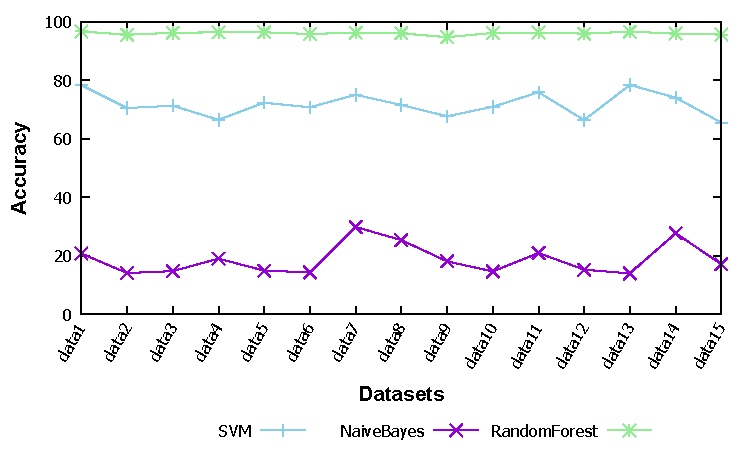
\includegraphics[width=\linewidth]{images/weka_accuracy3}
        \caption{Our attempt - Weka}
    \end{subfigure}%
    \begin{subfigure}[t]{0.4\textwidth}
        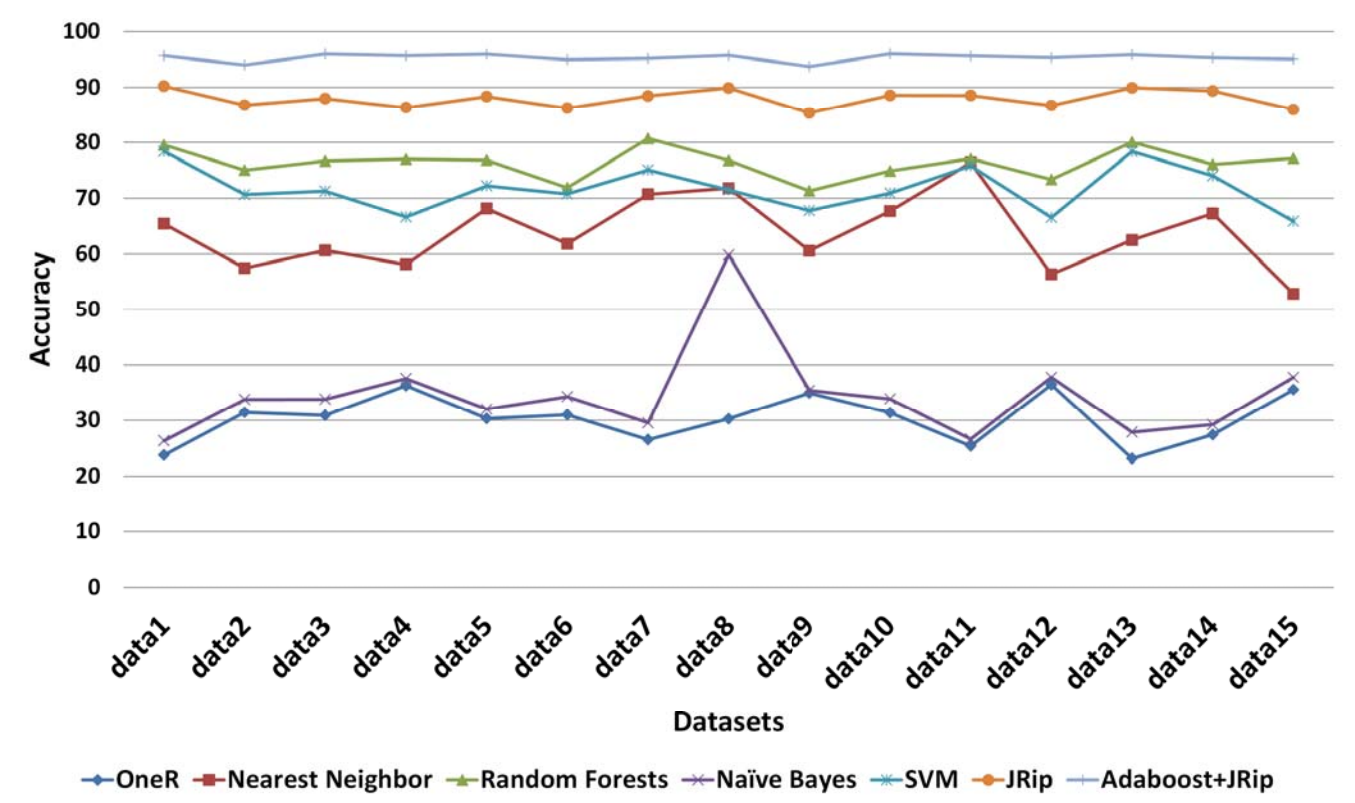
\includegraphics[width=\linewidth]{images/weka_accuracy3_cite.png}
        \caption{Original results \cite{borges_hink_machine_2014-1}}
    \end{subfigure}
    \begin{subfigure}[t]{0.4\textwidth}
        \includegraphics[width=\linewidth, page = 2]{images/accuracy}
        \caption{Our attempt - scikit-learn}
    \end{subfigure}
    \caption{Accuracy for three-class datasets}
    \label{fig:weka_acc3}
\end{figure}

\begin{figure}[H]
    \centering
    \begin{subfigure}[t]{0.4\textwidth}
        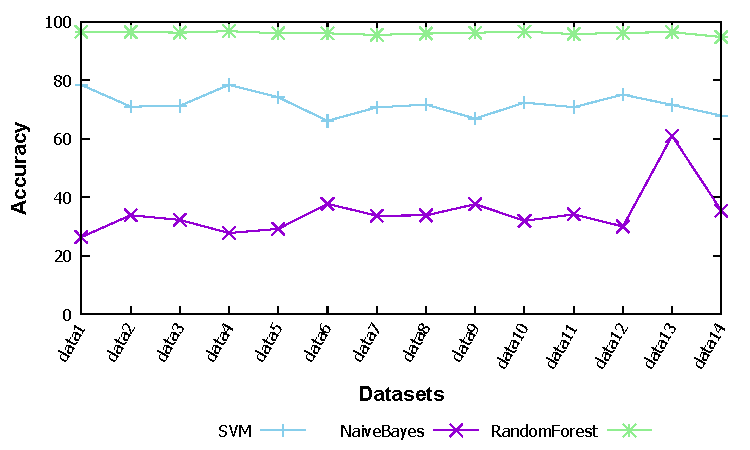
\includegraphics[width=\linewidth]{images/weka_accuracy2}
        \caption{Our attempt - Weka}
    \end{subfigure}%
    \begin{subfigure}[t]{0.4\textwidth}
        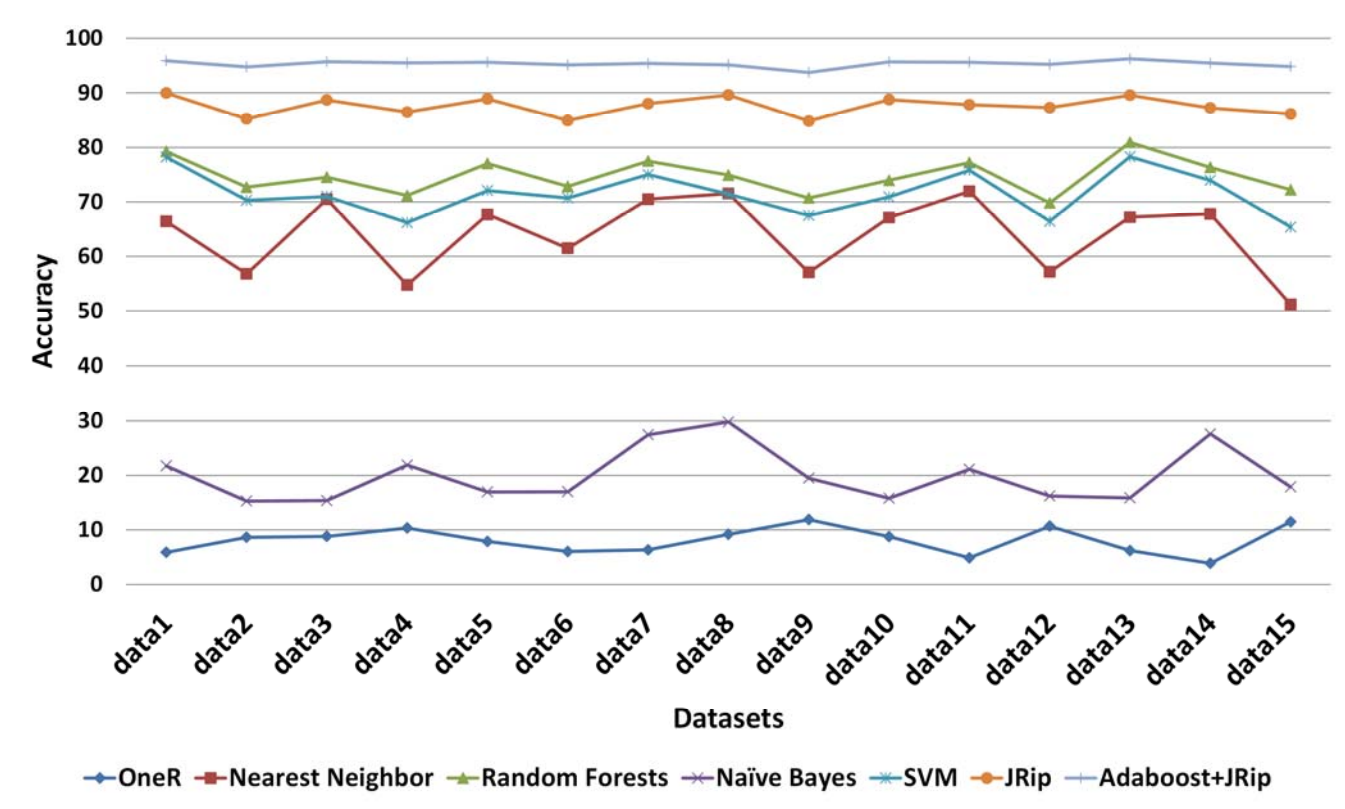
\includegraphics[width=\linewidth]{images/weka_accuracy2_cite.png}
        \caption{Original results \cite{borges_hink_machine_2014-1}}
    \end{subfigure}    
    \begin{subfigure}[t]{0.4\textwidth}
        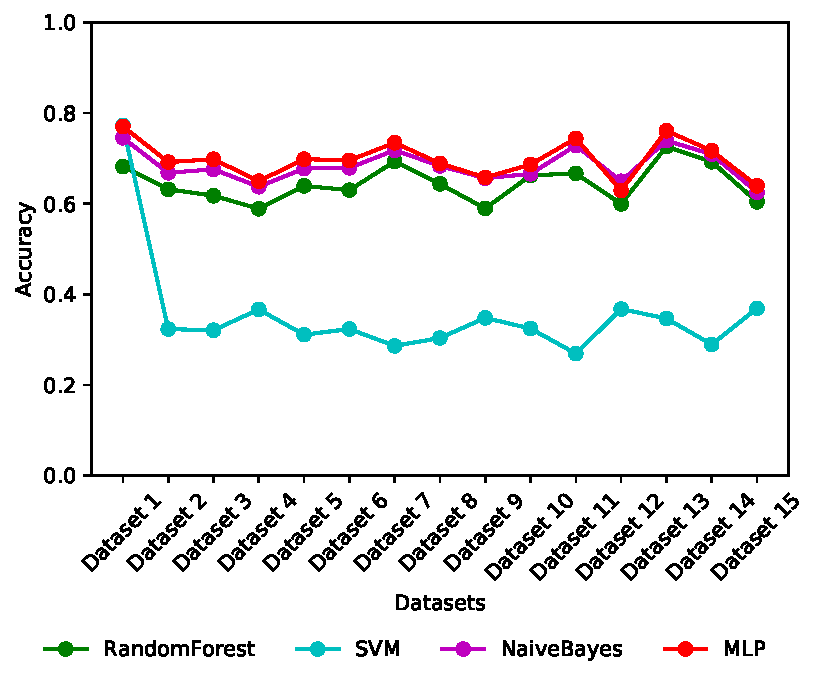
\includegraphics[width=\linewidth, page = 1]{images/accuracy}
        \caption{Our attempt - scikit-learn}
    \end{subfigure}
    \caption{Accuracy for binary datasets}
    \label{fig:weka_acc2}
\end{figure}

\begin{figure}[H]
    \centering
    \begin{subfigure}[t]{0.4\textwidth}
        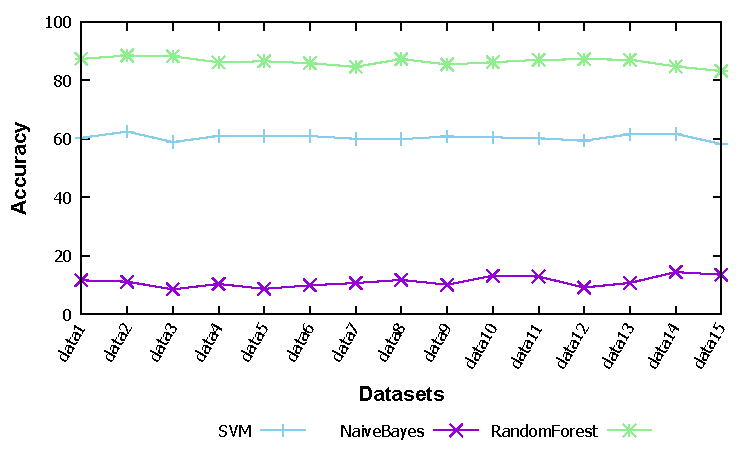
\includegraphics[width=\linewidth]{images/weka_accuracyall}
        \caption{Our attempt - Weka}
    \end{subfigure}%
    \begin{subfigure}[t]{0.4\textwidth}
        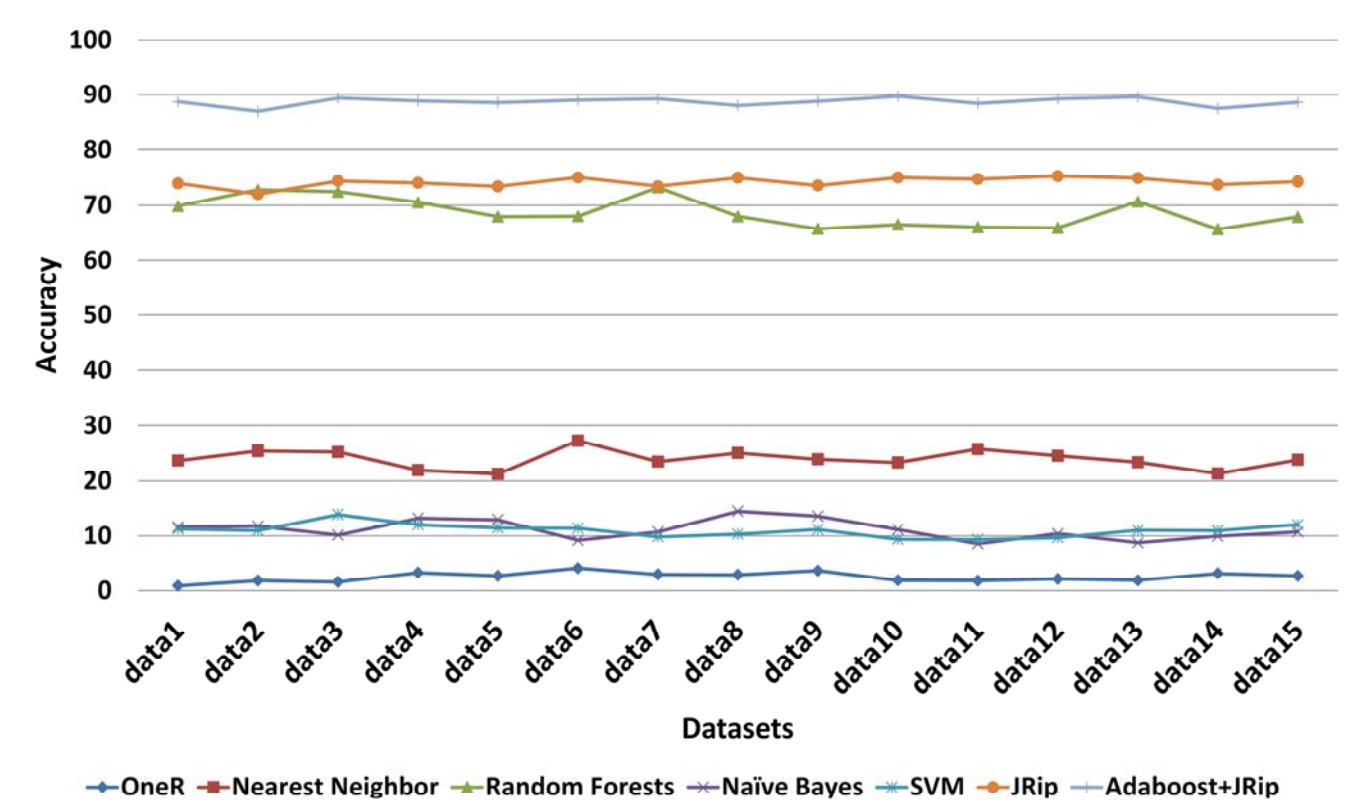
\includegraphics[width=\linewidth]{images/weka_accuracyall_cite.png}
        \caption{Original results \cite{borges_hink_machine_2014-1}}
    \end{subfigure}
    \begin{subfigure}[t]{0.4\textwidth}
        \includegraphics[width=\linewidth, page = 3]{images/accuracy}
        \caption{Our attempt - scikit-learn}
    \end{subfigure}
    \caption{Accuracy for multiclass datasets}
    \label{fig:weka_accall}
\end{figure}

\begin{figure}[H]
    \centering
    \begin{subfigure}[t]{0.4\textwidth}
        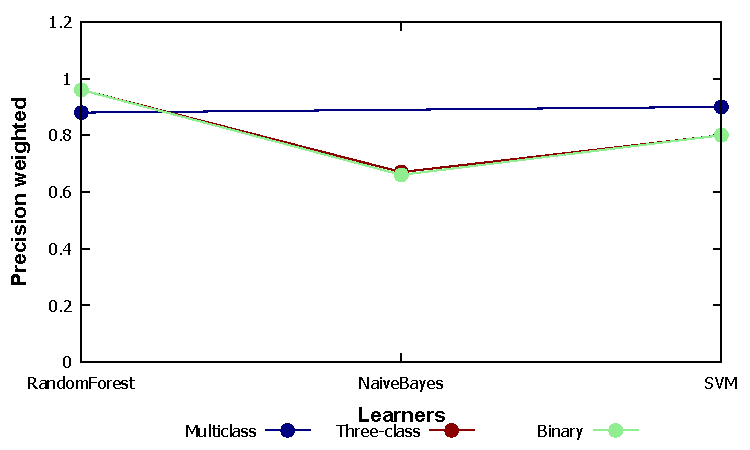
\includegraphics[width=\linewidth]{images/weka_precweight}
        \caption{Our attempt - Weka}
    \end{subfigure}%
    \begin{subfigure}[t]{0.4\textwidth}
        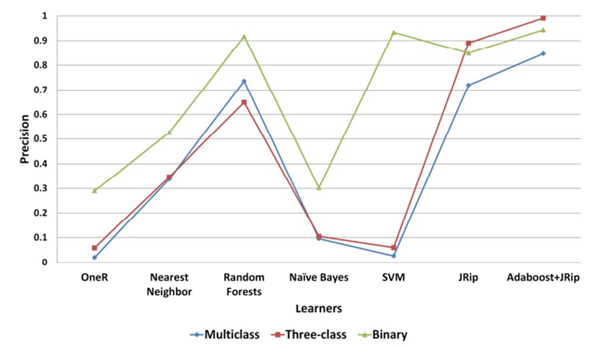
\includegraphics[width=\linewidth]{images/weka_precision_cite.png}
        \caption{Original results \cite{borges_hink_machine_2014-1}}
    \end{subfigure}
    \begin{subfigure}[t]{0.4\textwidth}
        \includegraphics[width=\linewidth, page = 3]{images/precision}
        \caption{Our attempt - scikit-learn}
    \end{subfigure}
    \caption{Precision}
    \label{fig:prec}
\end{figure}

\begin{figure}[H]
    \centering
    \begin{subfigure}[t]{0.4\textwidth}
        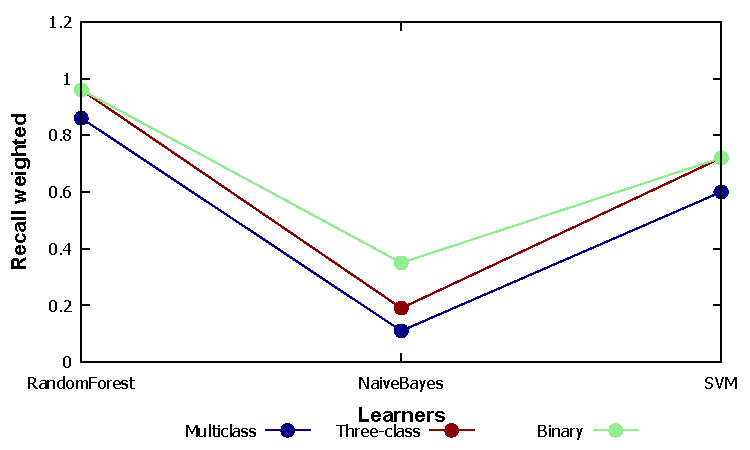
\includegraphics[width=\linewidth]{images/weka_recallweight}
        \caption{Our attempt - Weka}
    \end{subfigure}%
    \begin{subfigure}[t]{0.4\textwidth}
        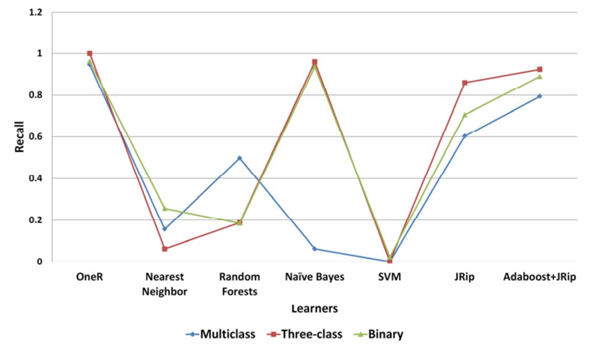
\includegraphics[width=\linewidth]{images/weka_recall_cite.png}
        \caption{Original results \cite{borges_hink_machine_2014-1}}
    \end{subfigure}
    \begin{subfigure}[t]{0.4\textwidth}
        \includegraphics[width=\linewidth, page = 3]{images/recall}
        \caption{Our attempt - scikit-learn}
    \end{subfigure}
    \caption{Recall}
    \label{fig:recall}
\end{figure}

\begin{figure}[H]
    \centering
    \begin{subfigure}[t]{0.4\textwidth}
        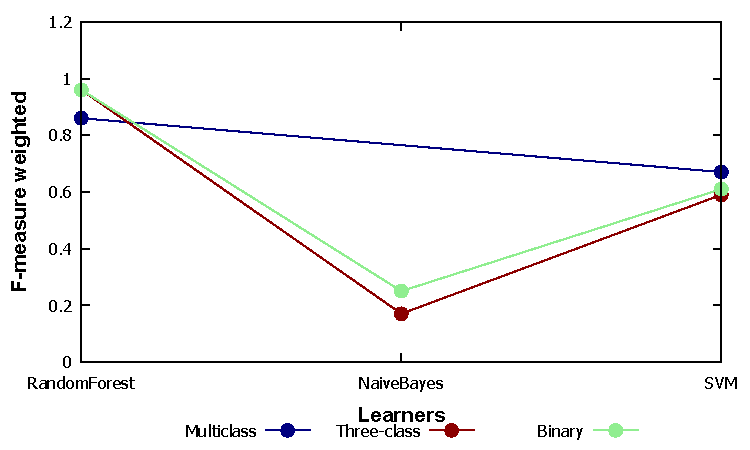
\includegraphics[width=\linewidth]{images/weka_f1weight}
        \caption{Our attempt - Weka}
    \end{subfigure}%
    \begin{subfigure}[t]{0.4\textwidth}
        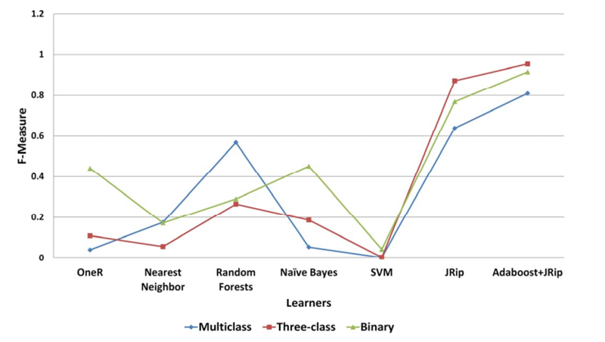
\includegraphics[width=\linewidth]{images/weka_f1_cite.png}
        \caption{Original results \cite{borges_hink_machine_2014-1}}
    \end{subfigure}
    \begin{subfigure}[t]{0.4\textwidth}
        \includegraphics[width=\linewidth, page = 3]{images/fmeasure}
        \caption{Our attempt - scikit-learn}
    \end{subfigure}  
    \caption{F-measure}
    \label{fig:f1}
\end{figure}

The accuracies in the three-class case are quite similar on the three plots, except SVM in scikit-learn, what shows a huge discrepancy of accuracy between datasets. Moreover, a remarkably higher values of accuracy for Random Forest classifier are observed in the attempt using Weka, compared to other plots.

In the binary and multiclass cases, the Random Forest classifier in the attempts using Weka always shows higher values comparable to other plots. Scikit-learn, on other hand, for Random Forest classifier, gives results similar to those made by \cite{borges_hink_machine_2014-1}. For SVM classifier, the discrepancy, this time, in the plots made by scikit-learn, is remarkably less important and the values oscillate around a constant value. For the binary case, this value is about 0.3 in scikit-learn, while in Weka the obtained value is 0.75, which makes it comparable to the original results in \cite{borges_hink_machine_2014-1}. On the other hand, in the multiclass case, the value oscillates around 0.1, like it is the case in the results from \cite{borges_hink_machine_2014-1}. In the attempt made in Weka the accuracy is much higher at about 0.6. For the NaïveBayes classifier the results are comparable, except the results obtained in scikit-learn in the binary case.

For precision, recall and f-measure, some similarities can be observed especially in the case of Random Forest classifier and in the case of NaïveBayes for multiclass. The results are generally different for the three metrics. For binary and multi-class cases the values of metrics are similar, except NaïveBayes classifier case. The most similar to the results from \cite{borges_hink_machine_2014-1} are the results obtained using scikit-learn, despite the differences. The more efficient classifier is certainly Random Classifier, especially when using Weka. However, MLP classifier gives also quite good results.

Moreover to get more information about the behaviour of the classifiers the f-measure macro and micro averages were calculated. The results are shown on figures \ref{fig:f1_macro}, \ref{fig:f1_micro} respectively. These metrics were not presented in \cite{borges_hink_machine_2014-1}.

\begin{figure}[H]
    \centering
    \begin{subfigure}[t]{0.5\textwidth}
        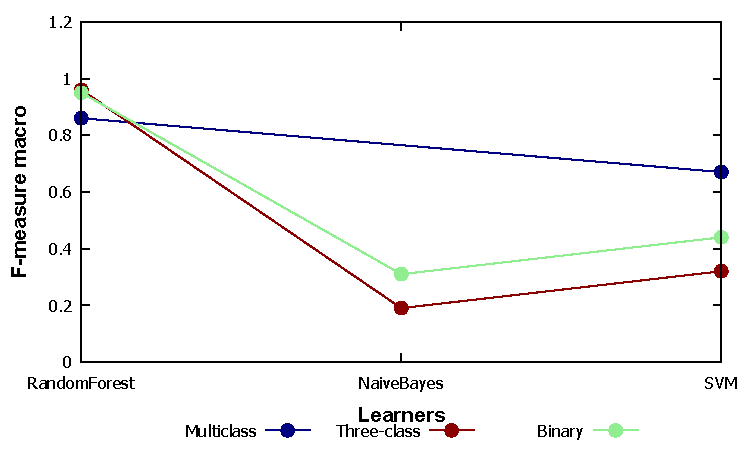
\includegraphics[width=\linewidth]{images/weka_f1macro}
        \caption{Weka}
    \end{subfigure}%
    \begin{subfigure}[t]{0.42\textwidth}
        \includegraphics[width=\linewidth, page = 2]{images/fmeasure}
        \caption{scikit-learn}
    \end{subfigure}
    \caption{F-measure macro}
    \label{fig:f1_macro}
\end{figure}

\begin{figure}[H]
    \centering
    \begin{subfigure}[t]{0.5\textwidth}
        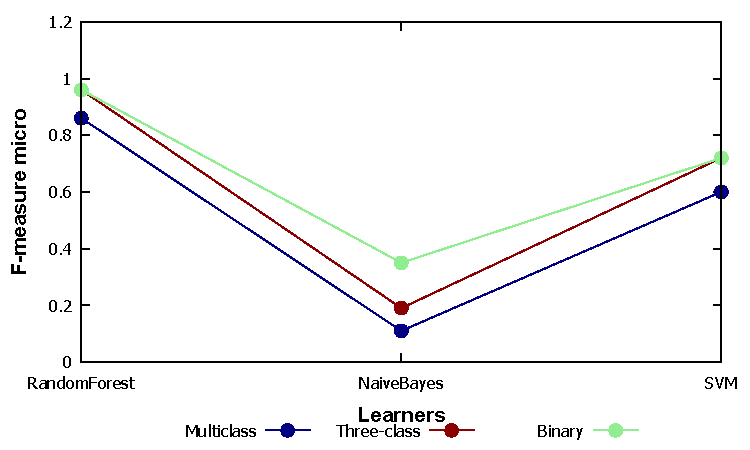
\includegraphics[width=\linewidth]{images/weka_f1micro}
        \caption{Weka}
    \end{subfigure}%
    \begin{subfigure}[t]{0.42\textwidth}
        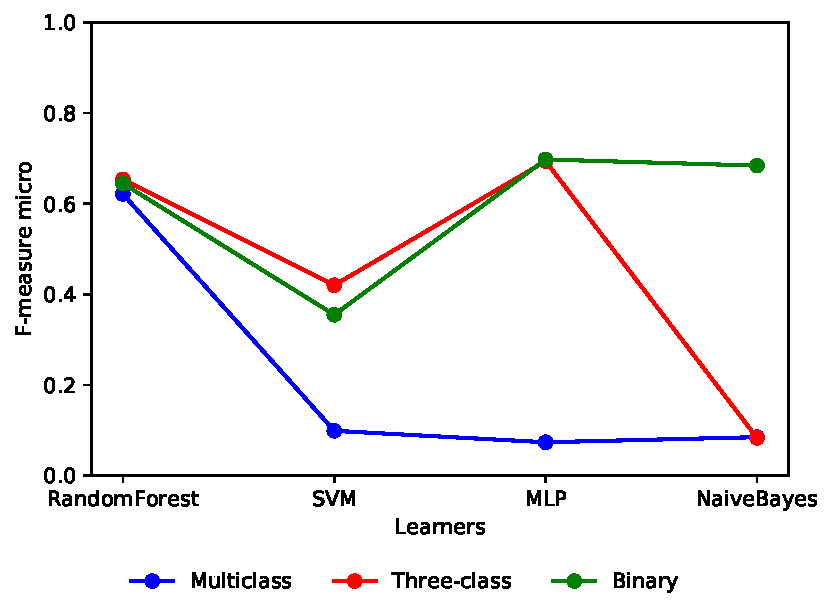
\includegraphics[width=\linewidth, page = 1]{images/fmeasure}
        \caption{scikit-learn}
    \end{subfigure}
    \caption{F-measure micro}
    \label{fig:f1_micro}
\end{figure}


It would be hard to say that the obtained results in Weka and scikit-learn are similar. These results confirm that Weka and scikit-learn tend to produce different results and that  results obtained by \cite{borges_hink_machine_2014-1} are hard to reproduce because of lack information about the used parameters by the author. Additionally, it may be concluded that the best classifier is Random Forest, followed by MLP, especially in binary and three-class cases. 

Since the results for three-class and binary cases were comparable and the three-class case gives more information about the status of the system, in what follows, the focus will be on the three-class case.

\section{scikit-learn further methods' analysis}

In addition to all that, scikit-learn enables the user to plot the receiver operating characteristic (ROC) curves for each class and the confusion matrix. The ROC curve represents the plot of true positive rate when the false positive rate changes. It is based on the prediction probabilities for each class given for each tested sample. Those predictions can be provided in two different ways:
\begin{itemize}
    \item concatenation of these probabilities for each cross-validation iteration,
    \item determination of probabilities for preselected test dataset values.
\end{itemize} 
The confusion matrix on the other hand shows the normalized number (over the total number of samples) of predicted values of each class for each class. The results are illustrated on figures \ref{fig:ROCCM_RF}, \ref{fig:ROCCM_SVM}, \ref{fig:ROCCM_NB} and \ref{fig:ROCCM_MLP}.

\begin{figure}[H]
    \centering
    \begin{subfigure}[t]{0.33\textwidth}
        \centering
        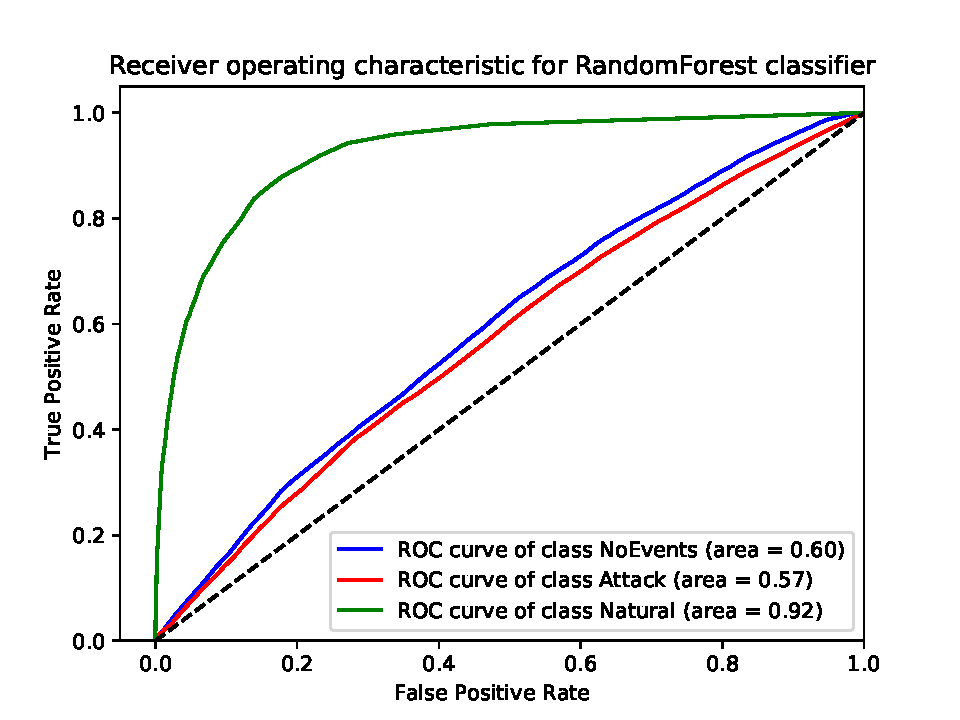
\includegraphics[page=1, width=\linewidth]{images/results_scikit/RandomForest}
        \caption{ROC Curve - cross-validation}
        \label{fig:scikit_RF_ROC}
    \end{subfigure}
    \begin{subfigure}[t]{0.33\textwidth}
        \centering
        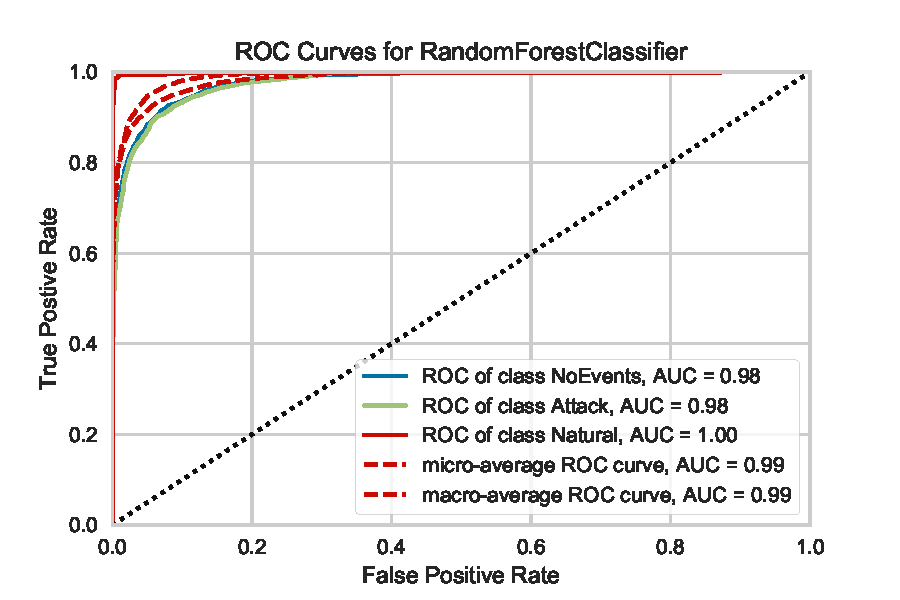
\includegraphics[page=1, width=\linewidth]{images/roc_3c}
        \caption{ROC Curve}
        \label{fig:scikit_RF_ROC}
    \end{subfigure}
    \begin{subfigure}[t]{0.3\textwidth}
        \centering
        \includegraphics[page=2, width=\linewidth, trim= 0 50 0 100, clip]{images/results_scikit/RandomForest}
        \caption{Confusion Matrix}
        \label{fig:scikit_RF_CM}
    \end{subfigure}
    \caption{Random Forest ROC curve and confusion matrix}
    \label{fig:ROCCM_RF}
\end{figure}

\begin{figure}[H]
    \centering
    \begin{subfigure}[t]{0.33\textwidth}
        \centering
        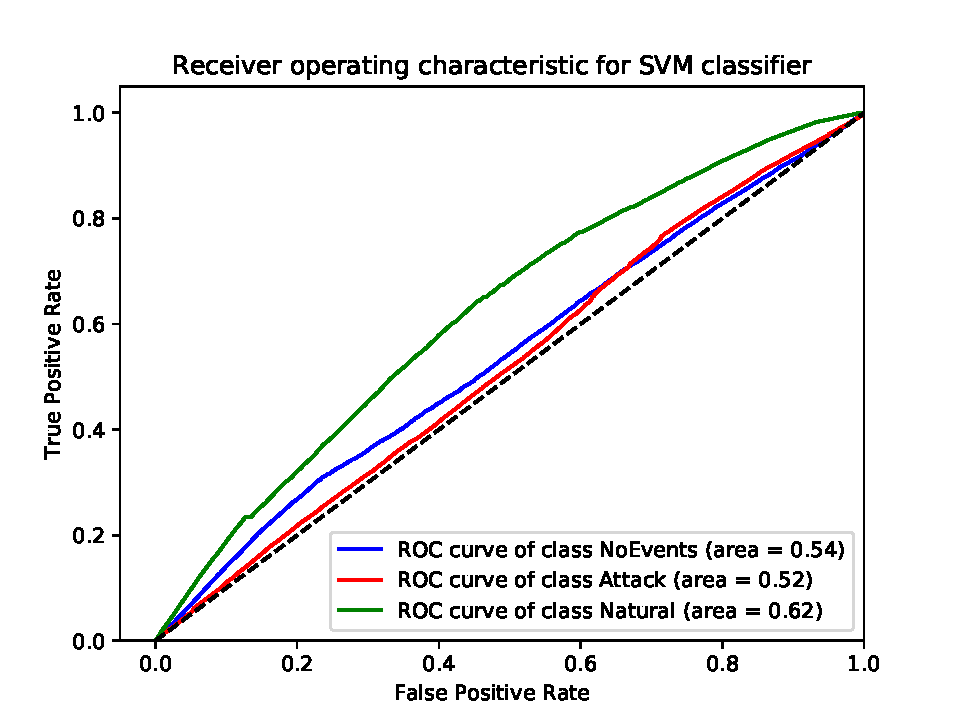
\includegraphics[page=1, width=\linewidth]{images/results_scikit/SVM}
        \caption{ROC Curve - cross-validation}
        \label{fig:scikit_SVM_ROC}
    \end{subfigure}
    \begin{subfigure}[t]{0.33\textwidth}
        \centering
        \includegraphics[page=2, width=\linewidth]{images/roc_3c}
        \caption{ROC Curve}
        \label{fig:scikit_RF_ROC}
    \end{subfigure}
    \begin{subfigure}[t]{0.3\textwidth}
        \centering
        \includegraphics[page=2, width=\linewidth, trim= 0 50 0 100, clip]{images/results_scikit/SVM}
        \caption{Confusion Matrix}
        \label{fig:scikit_SVM_CM}
    \end{subfigure}
    \caption{SVM ROC curve and confusion matrix}
    \label{fig:ROCCM_SVM}
\end{figure}

\begin{figure}[H]
    \begin{subfigure}[t]{0.33\textwidth}
        \centering
        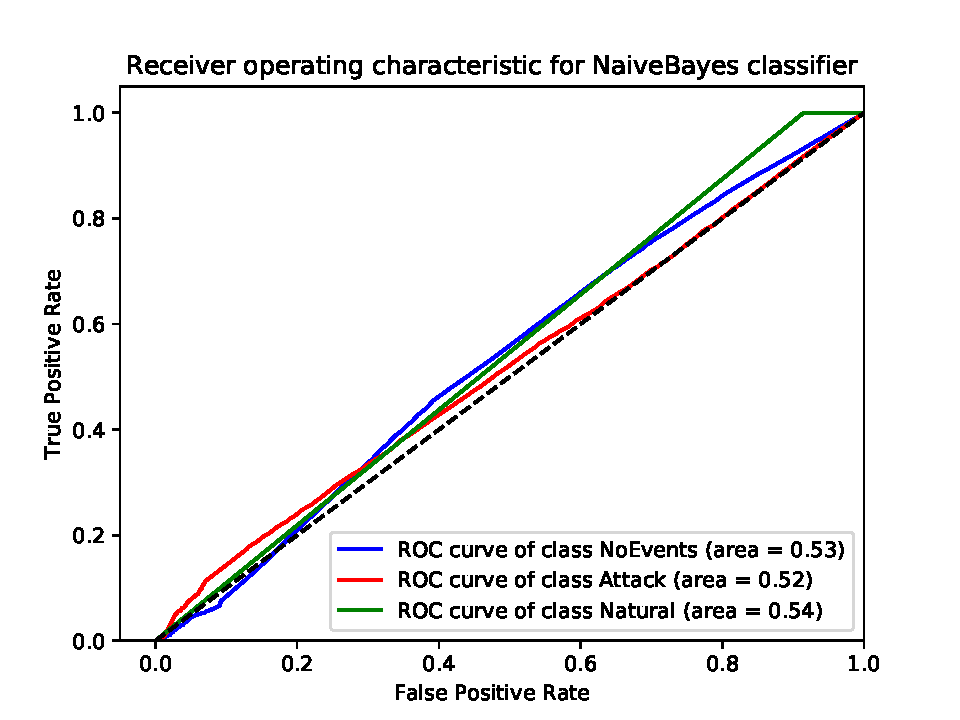
\includegraphics[page=1, width=\linewidth]{images/results_scikit/NaiveBayes}
        \caption{ROC Curve - cross-validation}
        \label{fig:scikit_NB_ROC}
    \end{subfigure}
    \begin{subfigure}[t]{0.33\textwidth}
        \centering
        \includegraphics[page=4, width=\linewidth]{images/roc_3c}
        \caption{ROC Curve}
        \label{fig:scikit_RF_ROC}
    \end{subfigure}
    \begin{subfigure}[t]{0.3\textwidth}
        \centering
        \includegraphics[page=2, width=\linewidth, trim= 0 50 0 100, clip]{images/results_scikit/NaiveBayes}
        \caption{Confusion Matrix}
        \label{fig:scikit_NB_CM}
    \end{subfigure}
    \caption{Naïve Bayes ROC curve and confusion matrix}
    \label{fig:ROCCM_NB}
\end{figure}

\begin{figure}[H]
    \begin{subfigure}[t]{0.33\textwidth}
        \centering
        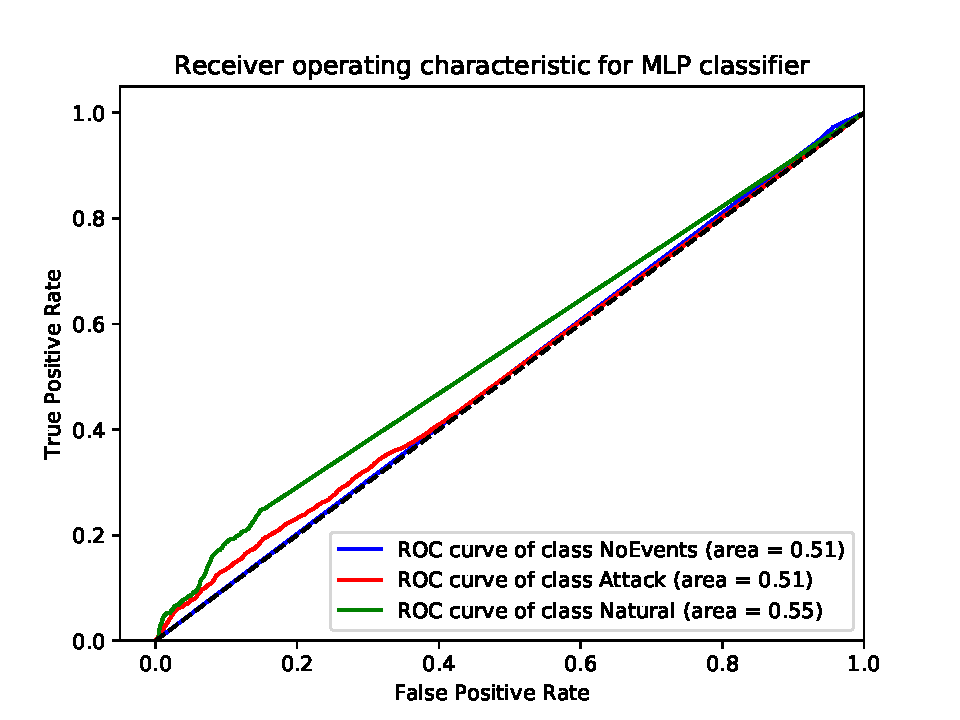
\includegraphics[page=1, width=\linewidth]{images/results_scikit/MLP}
        \caption{ROC Curve - cross-validation}
        \label{fig:scikit_MLP_ROC}
    \end{subfigure}
    \begin{subfigure}[t]{0.33\textwidth}
        \centering
        \includegraphics[page=3, width=\linewidth]{images/roc_3c}
        \caption{ROC Curve}
        \label{fig:scikit_RF_ROC}
    \end{subfigure}
    \begin{subfigure}[t]{0.3\textwidth}
        \centering
        \includegraphics[page=2, width=\linewidth, trim= 0 50 0 100, clip]{images/results_scikit/MLP}
        \caption{Confusion Matrix}
        \label{fig:scikit_MLP_CM}
    \end{subfigure}
    \caption{MLP ROC curve and confusion matrix}
    \label{fig:ROCCM_MLP}
\end{figure}

The previous figures show that Random Forest classifier has the higher capacities to distinguish between the occurrence of each class, or its absence. SVM tends to predict only NoEvents and Attacks but does not really succeed in distinguishing between them. Naïve Bayes fails to make true predictions, it considers everything of class natural. Finally MLP, it succeeds in determining the class NoEvents, but does not distinguish over classes almost at all, despite the high accuracy (it is due because of the huge number of samples of class NoEvents).

The two methods of plotting the ROC curve does not give exactly the same results, however the conclusions remain the same in both cases. This fact may be due to a slightly different set of test data used for its creation.

Given this analysis, it can be deducted that Random Forest algorithm acts the best, and that is why it will be adapted in next chapters, in which, at first, an analysis of features and their importance will be made. However a deeper look at the amelioration of  will be also made, in order to succeed in differentiation between the classes.


\chapter{Features' importance}

After having determined the most performant algorithm, which is Random Forest, it is time to go further and analyse which features impact the results of classification the most. The focus will be especially on false predictions. In order to do that, six tools will be compared: LIME \cite{lime}, ELI5 \cite{mikhail_korobov_eli5_nodate}, YellowBrick \cite{bengfort_yellowbrick_2018}, Treeinterpreter \cite{ando_saabas_treeinterpreter_nodate}, dtreeviz \cite{terence_parr_dtreeviz_nodate} and export\_graphviz tool from scikit-learn, where the last three ones are designed for Decision Tree and Random Forest classifiers.

\section{Result's interpreters' comparison}
\subsection{LIME} 
LIME (Local Interpretable Model-agnostic Explanations) is a tool that is used to explain the behaviour of machine learning classifiers. It supports, as for this day, only the explanation of individual predictions for any scikit-learn classifier or regressor. This explanation consist in a list of features (and more precisely decision nodes composed of feature name and a numeric condition) ordered by their relative importance for a particular prediction. This list can be shown is a raw mode (as a python list) or in a visual form (pyplot figure, jupyter notebook or html file).

In order to class the features according to their importance, LIME approximates the model by an interpretable one, created based on perturbing the features of the examined instance. More the perturbed instances are similar to the examined instance, higher is the weight of the perturbed feature. This approximation process is called explanation and is described using the following equation:

\begin{equation}
    \xi(x) = \operatorname*{argmin}_{g \in G} \mathcal{L}(f, g, \pi_x) + \Omega(g)\quad\cite{lime},
\end{equation}

\noindent where $g$ is the explanation model from the set of interpretable models $G$, $f$ is the probability that the sample $x$ corresponds to a certain class, $\pi_x$ is the distance between an instance $z$ and the sample~$x$. $\mathcal{L}(f, g, \pi_x)$ describes to which extent $g$ is unfaithful in the approximation of $f$ in the neighbourhood defined by $\pi_x$, while $\Omega(g)$ describes the complexity of the explanation (for example the depth of the tree if $f$ is a decision tree). The goal of the explanation is to find the most faithful approximation of $f$ taking into consideration the neighbourhood $\pi_x$.

To better illustrate the algorithm, let the pigeon image on figure \ref{fig:limepigeon} be considered as a sample used in a classification problem based on a classifier noted \textit{f}. The image can be divided into several regions, like it is shown on figure \ref{fig:limediv}, each region corresponds to a feature.

\begin{minipage}{.45\textwidth}
    \begin{figure}[H]
        \centering
        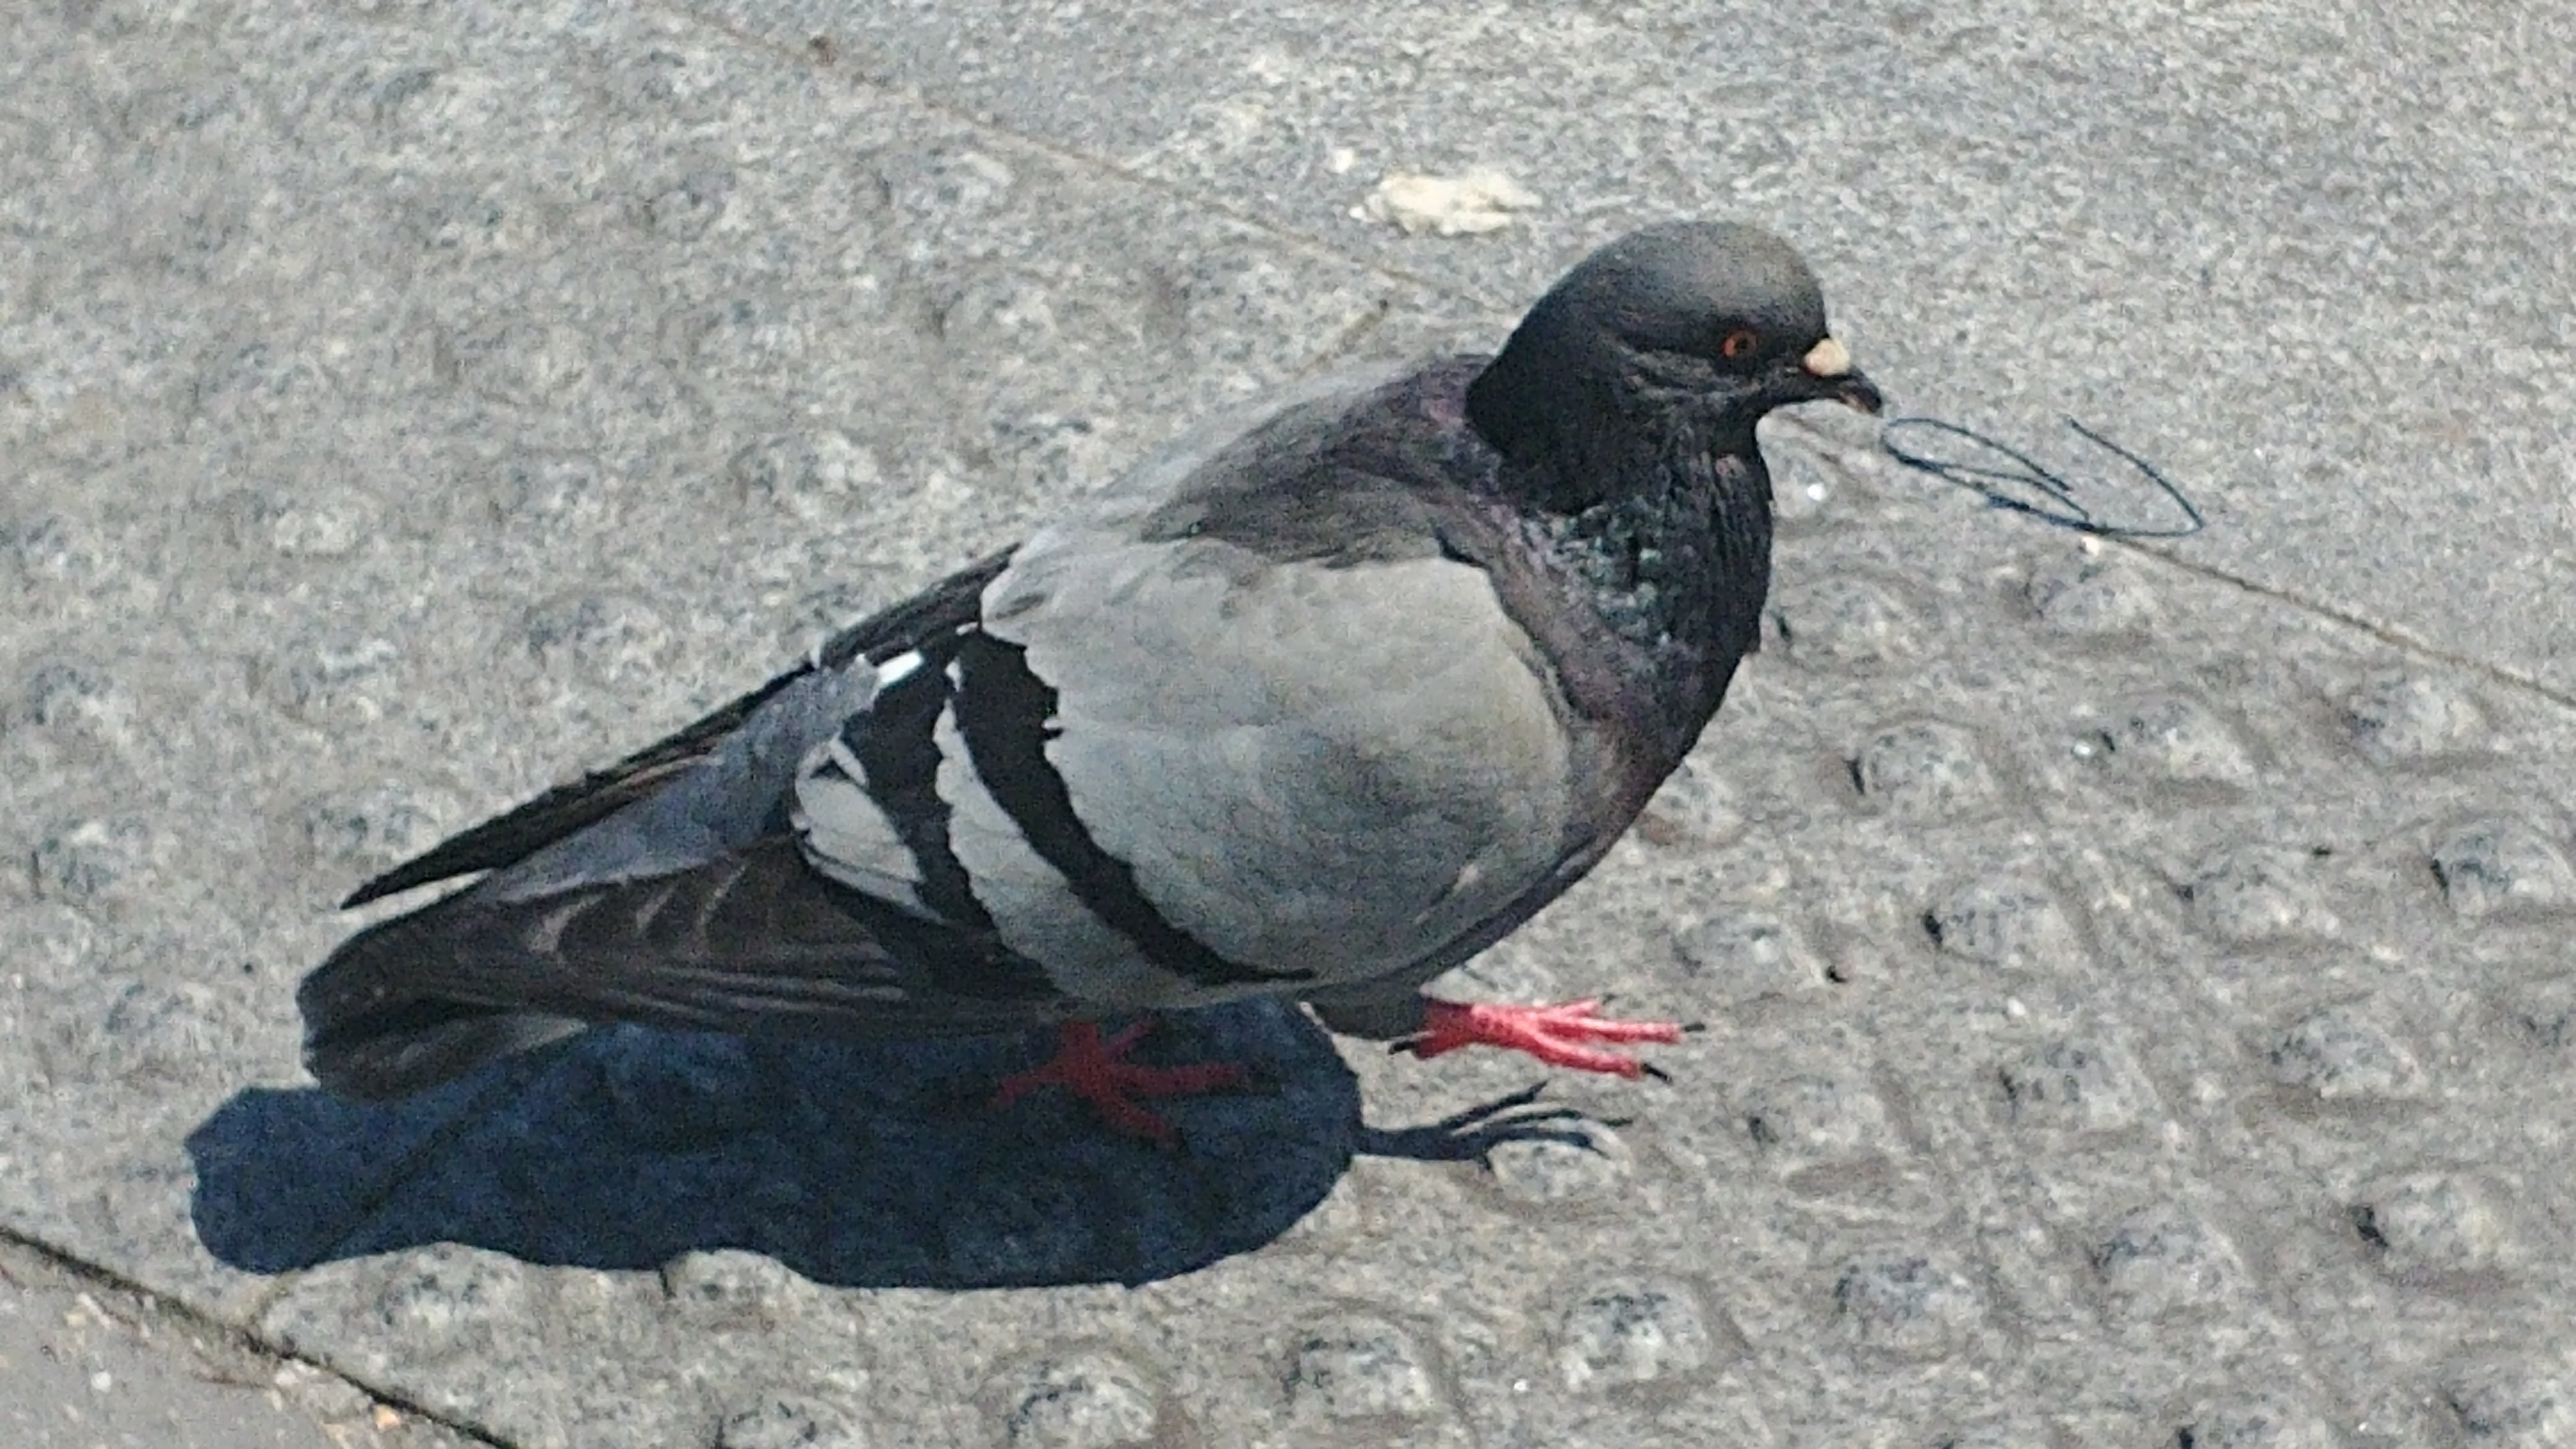
\includegraphics[width=\linewidth]{images/lime/pigeon}
        \caption{Pigeon}
        \label{fig:limepigeon}
    \end{figure}
\end{minipage}
\begin{minipage}{.45\textwidth}
    \begin{figure}[H]
        \centering
        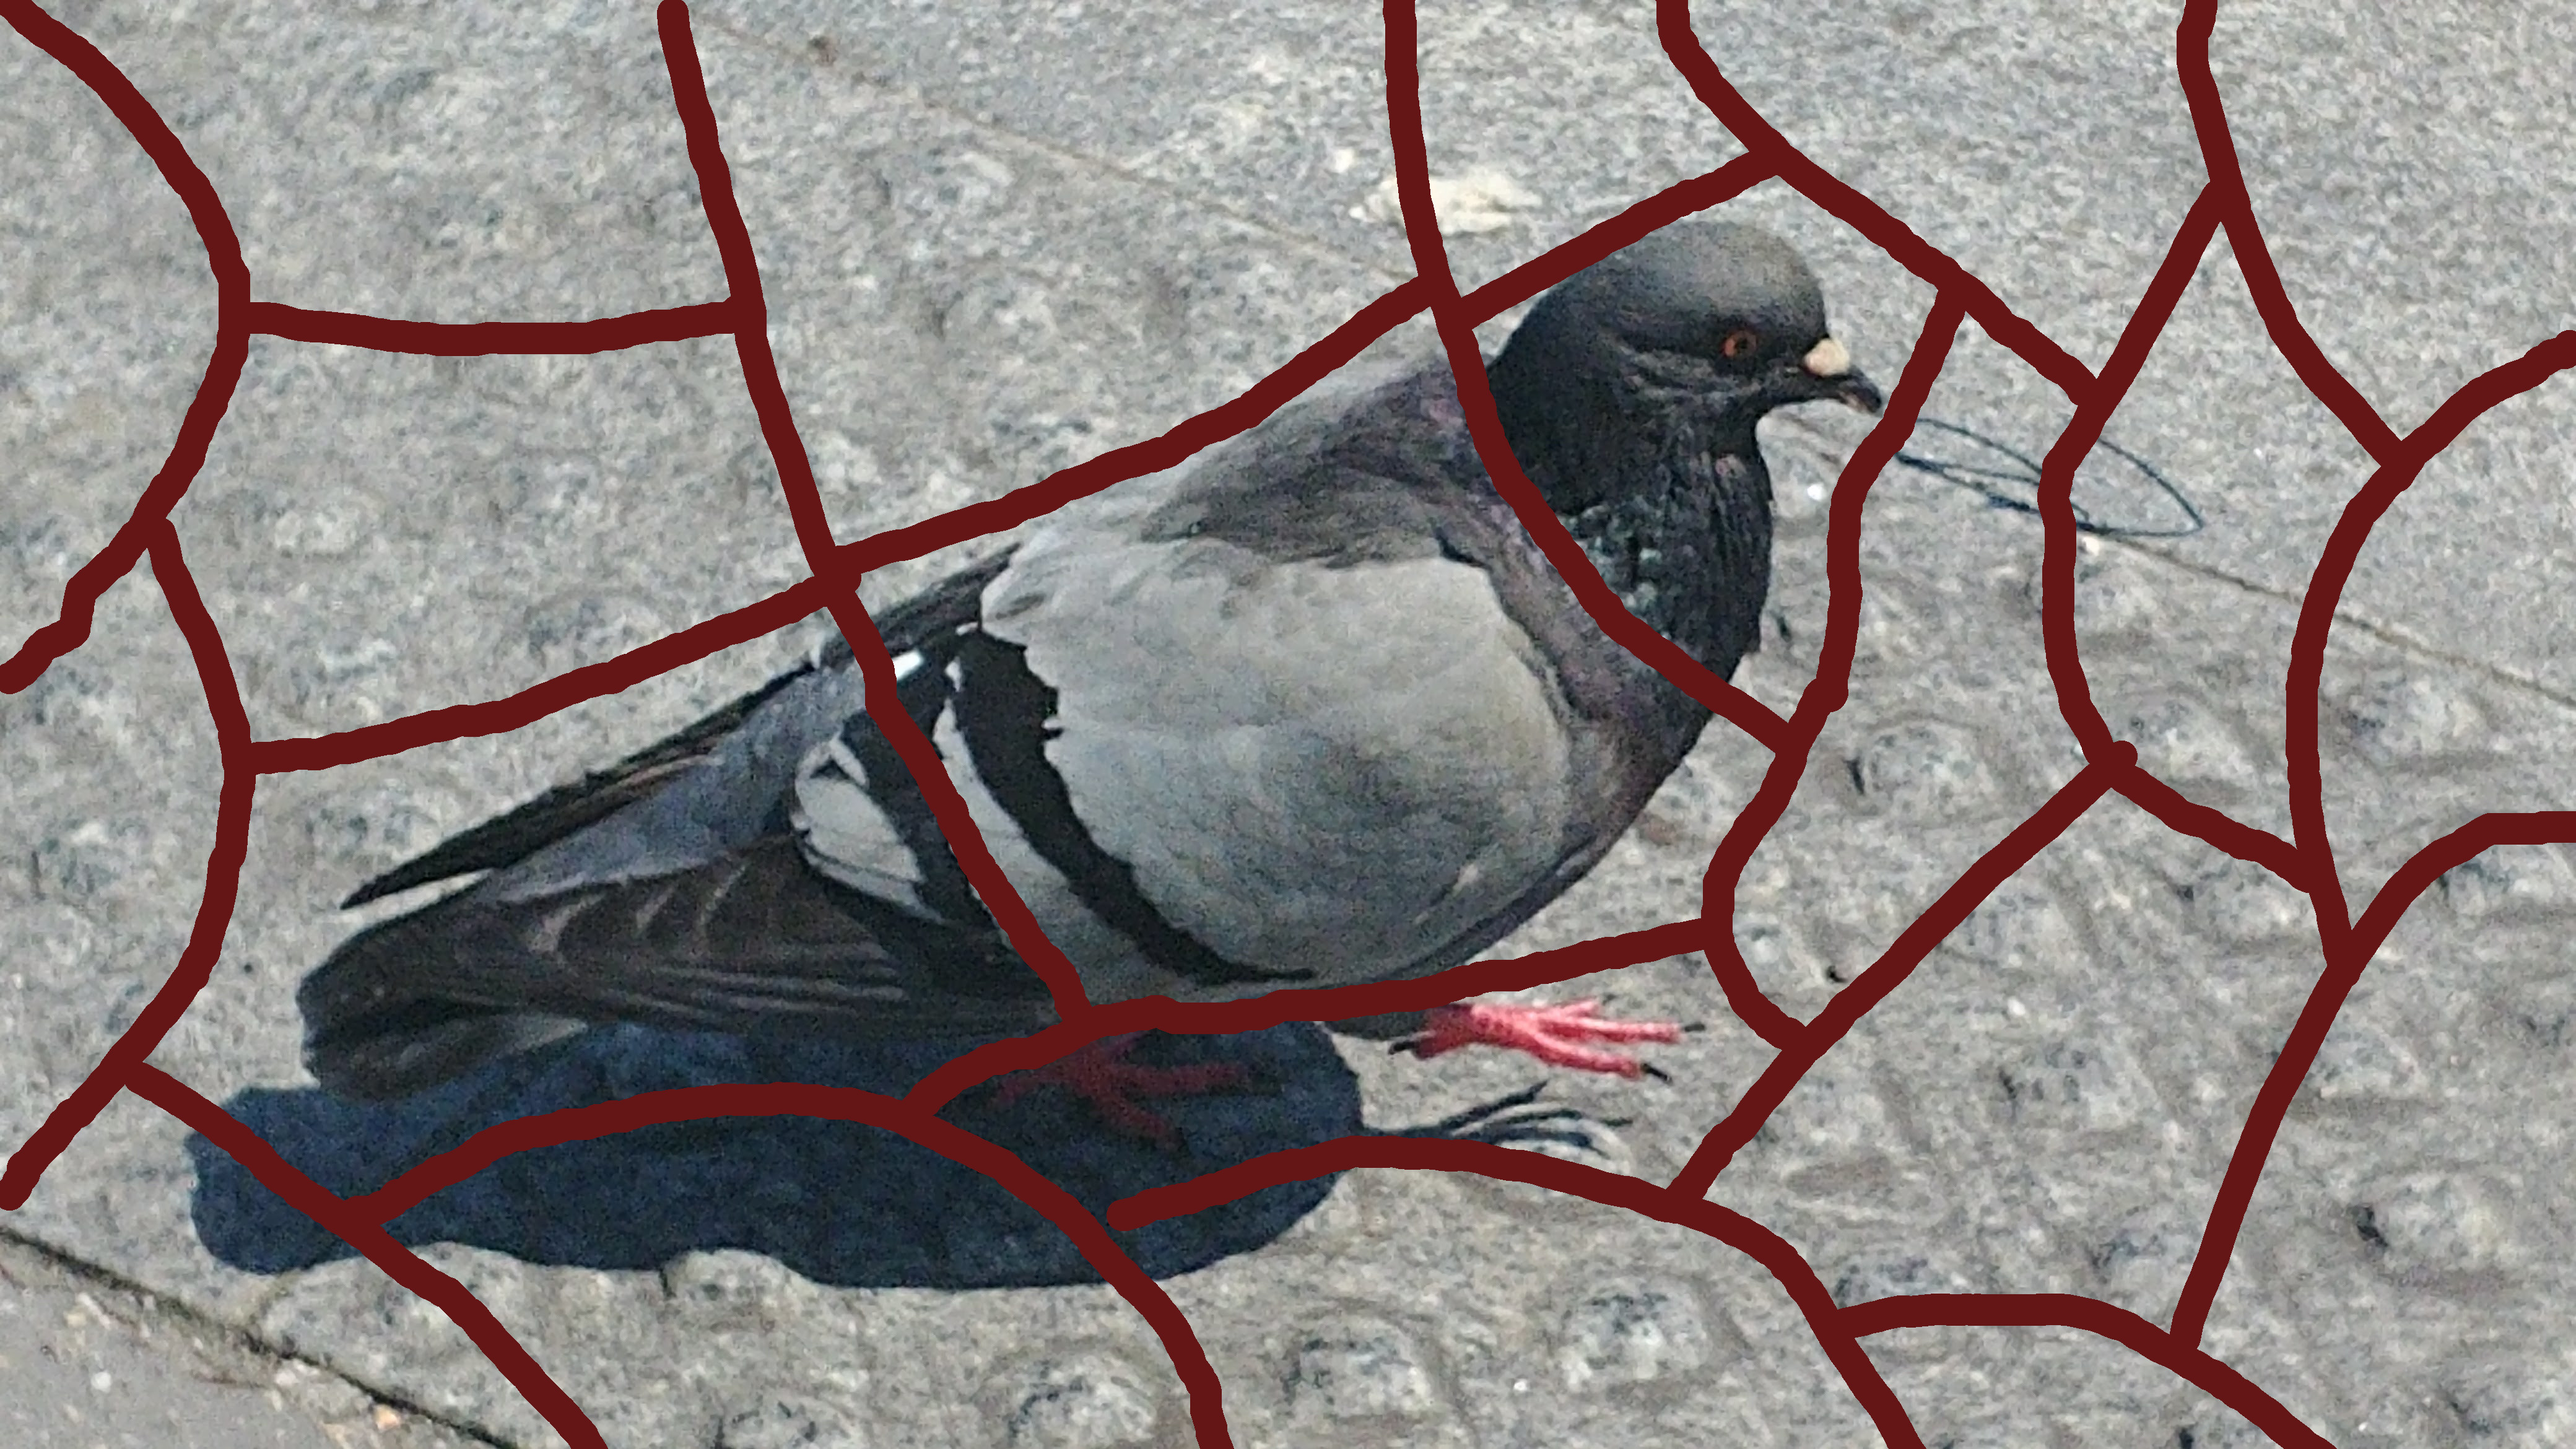
\includegraphics[width=\linewidth]{images/lime/grid}
        \caption{Image grid}
        \label{fig:limediv}
    \end{figure}
\end{minipage}
\vspace{0.5cm}

In the next step, a new dataset is created by modifying the features. In the case of the pigeon image some regions can be simply greyed out like it is shown on figure \ref{fig:limegrey}. For each of these regions the probability if it represents a pigeon or not is calculated using the classifier \textit{f}.

\begin{figure}[H]
    \centering
    \begin{subfigure}[t]{0.32\linewidth}
        \centering
        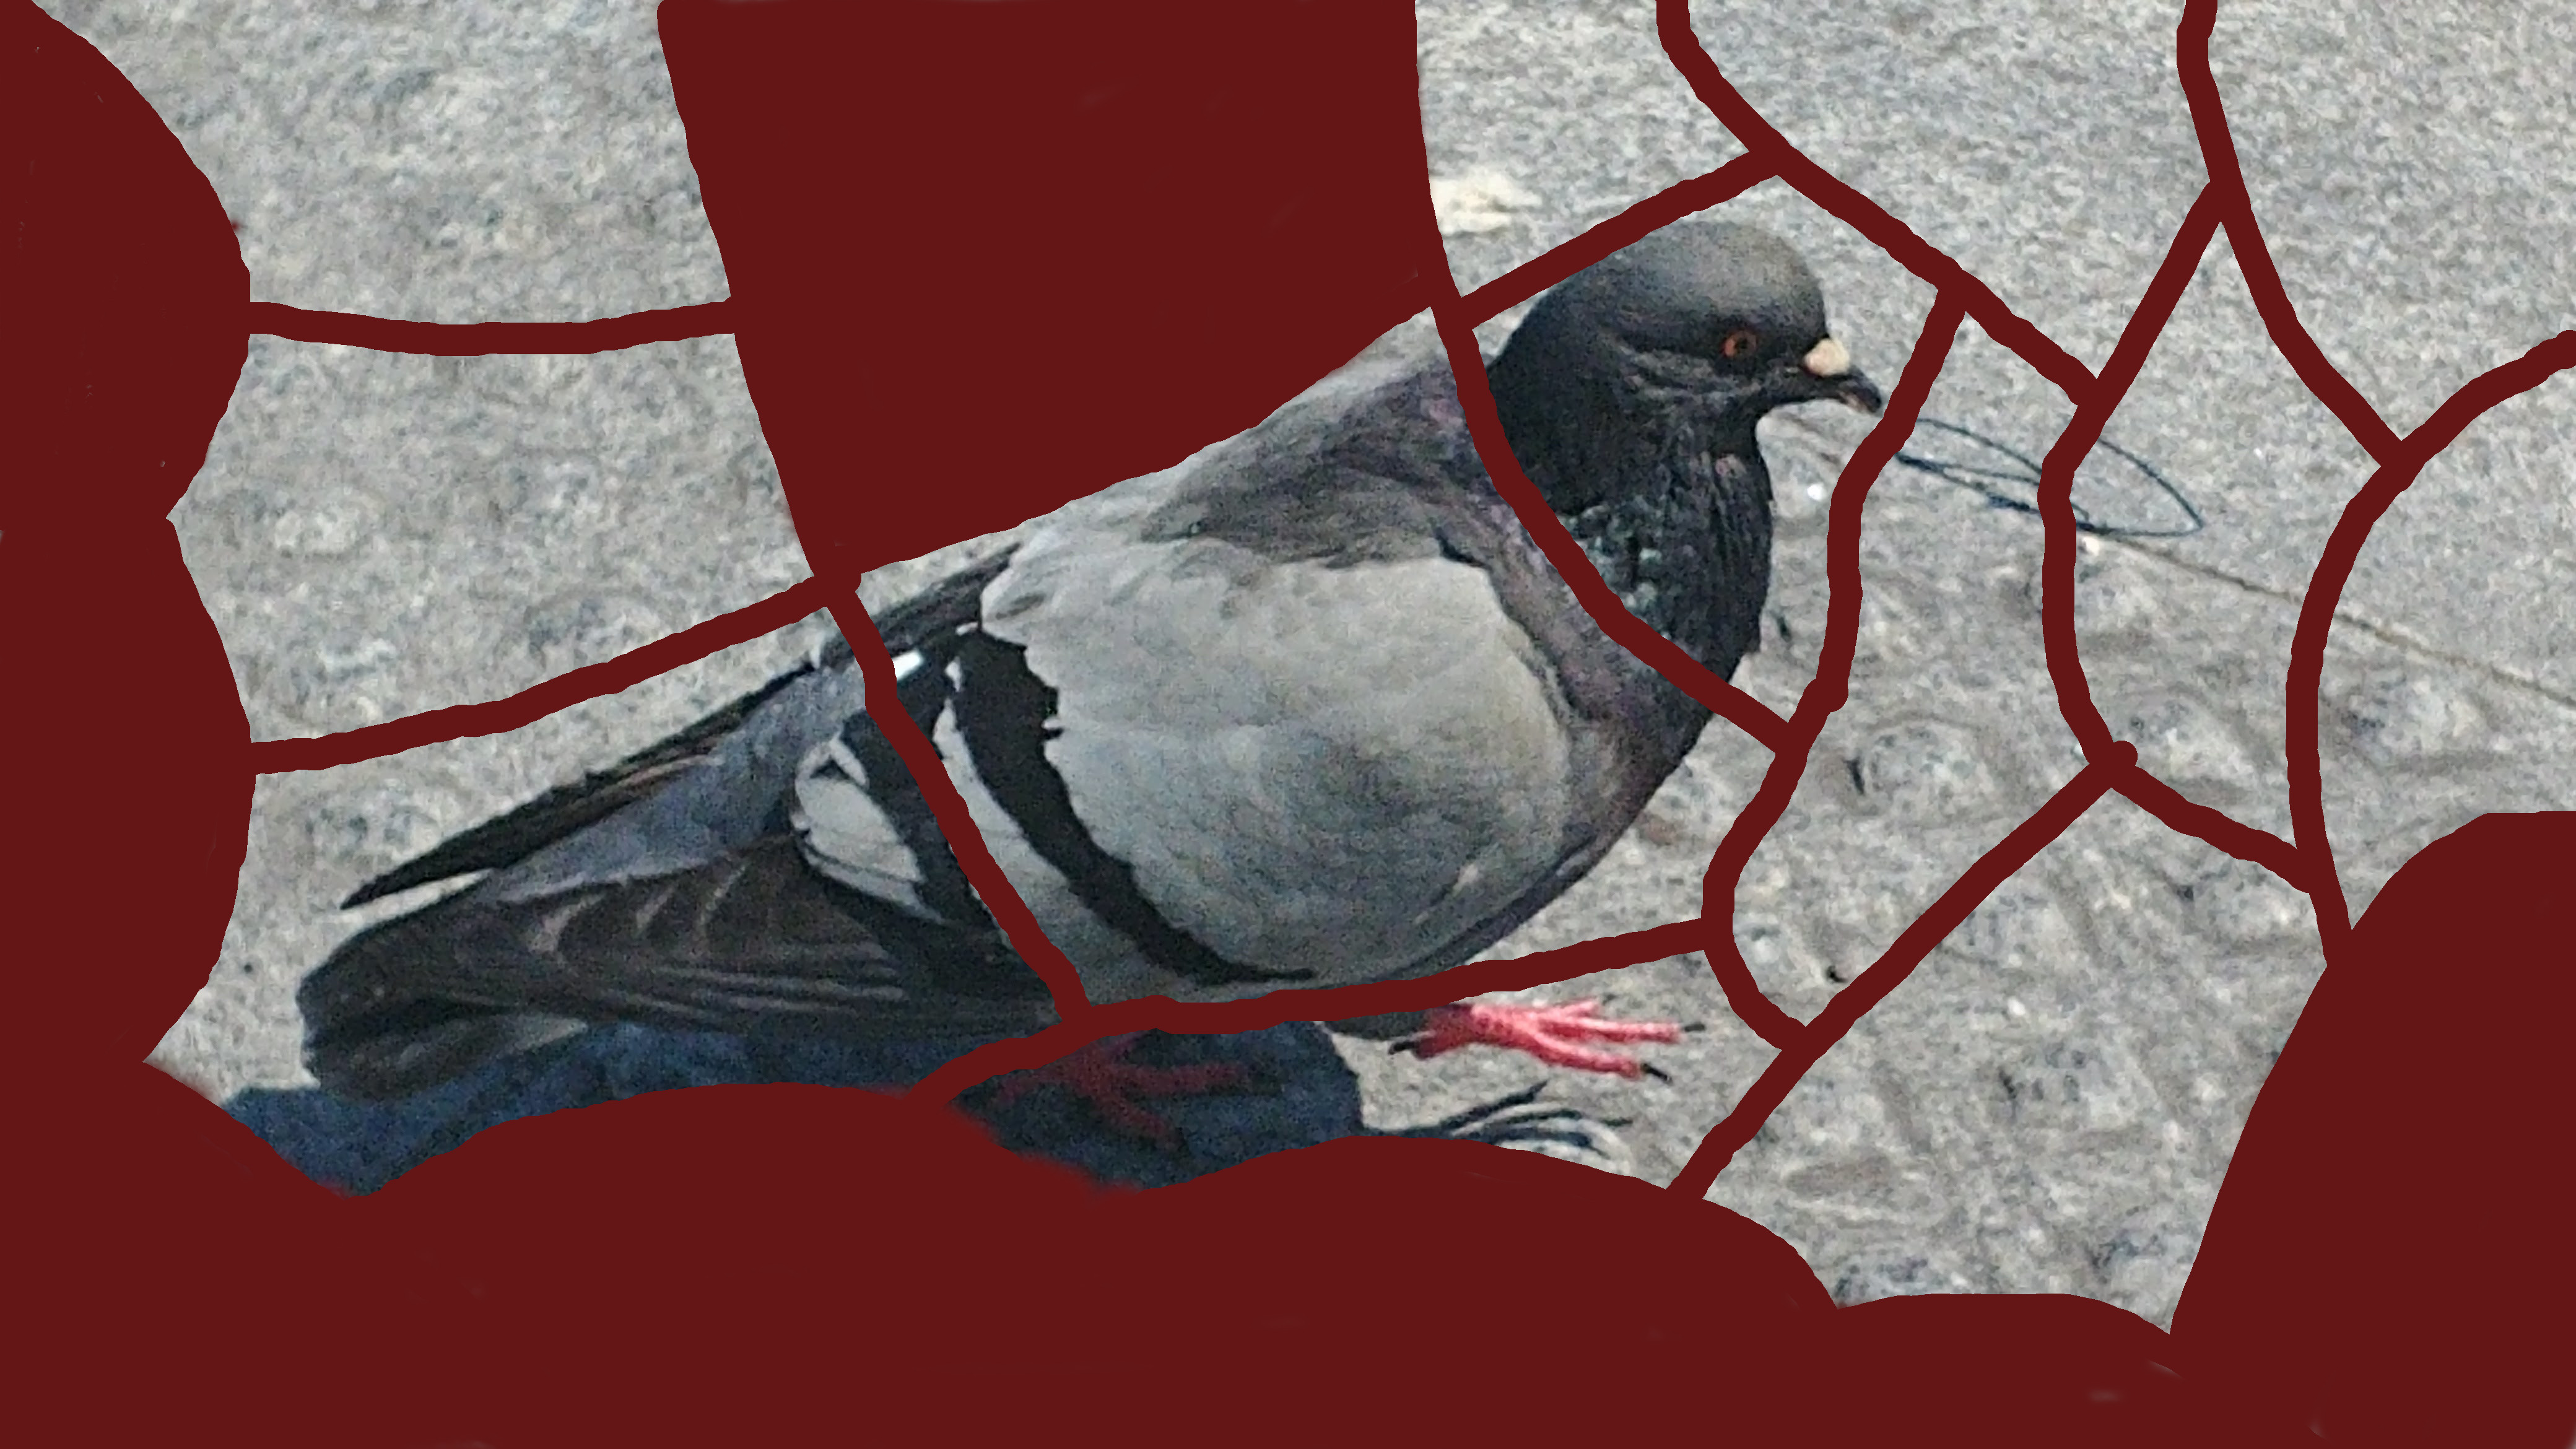
\includegraphics[width=\linewidth]{images/lime/pert1}
        \caption{Perturbation 1}
    \end{subfigure}
    \begin{subfigure}[t]{0.32\linewidth}
        \centering
        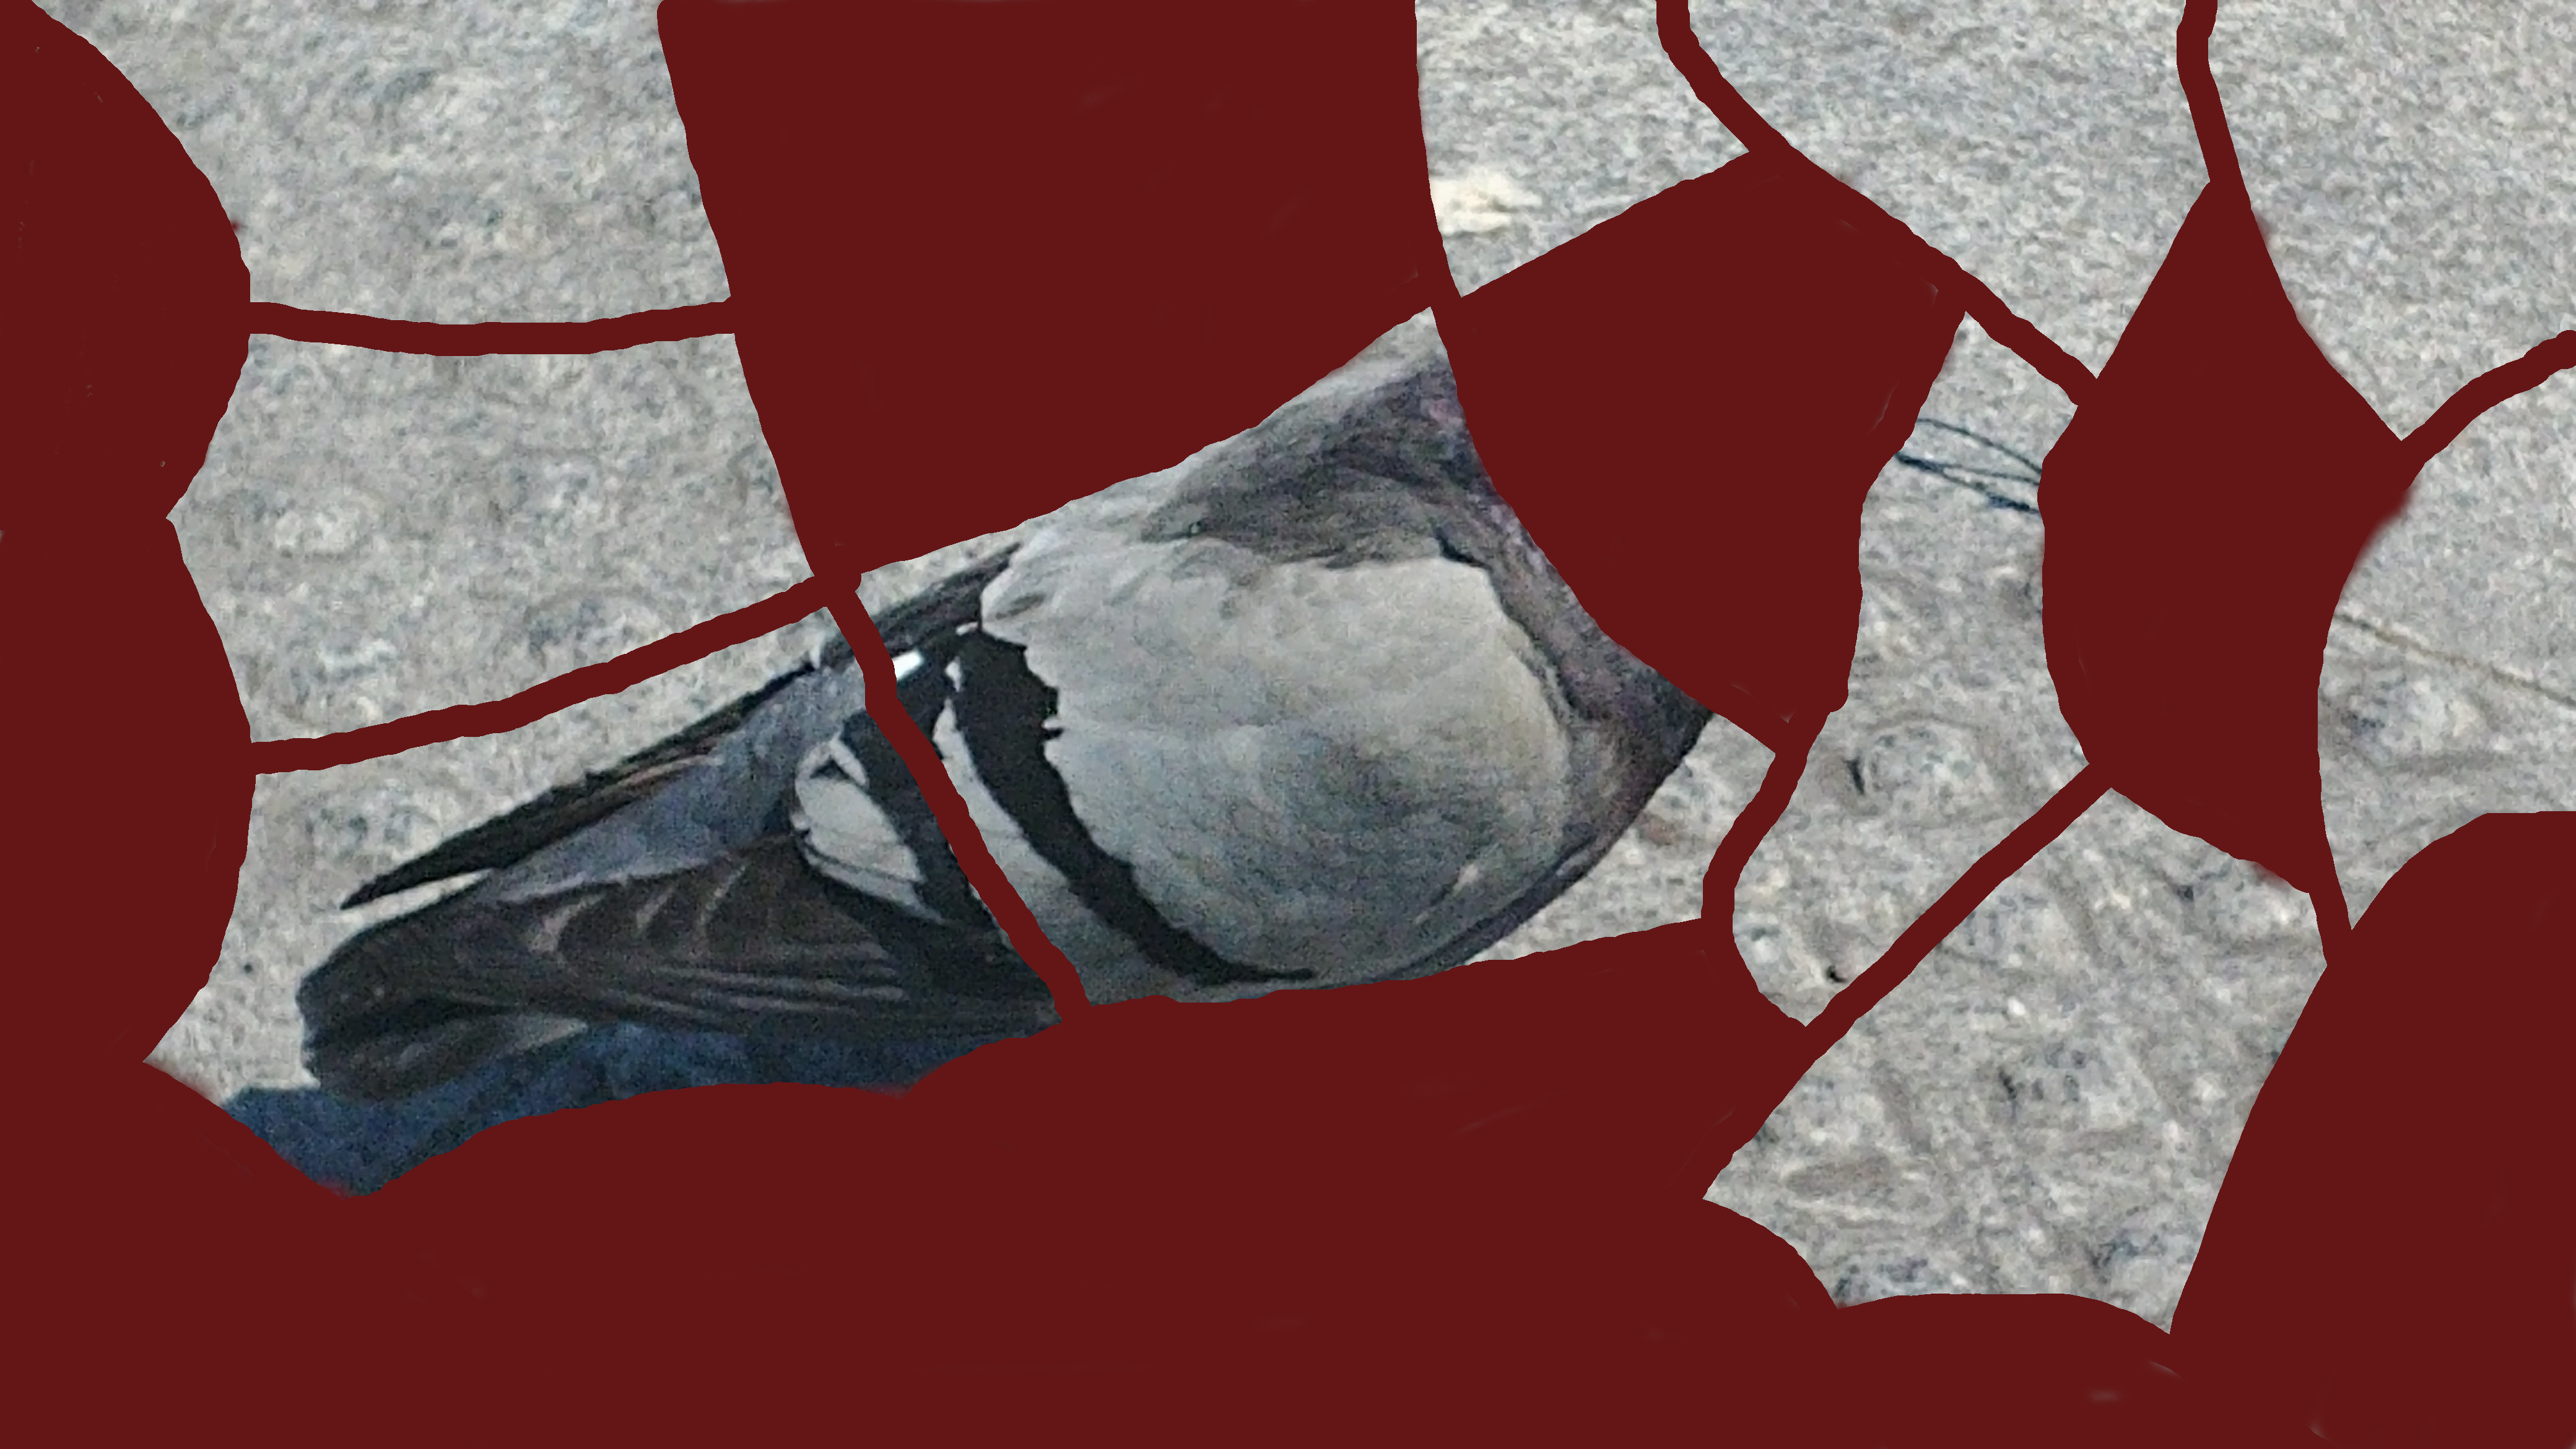
\includegraphics[width=\linewidth]{images/lime/pert2}
        \caption{Perturbation 2}
    \end{subfigure}
    \begin{subfigure}[t]{0.32\linewidth}
        \centering
        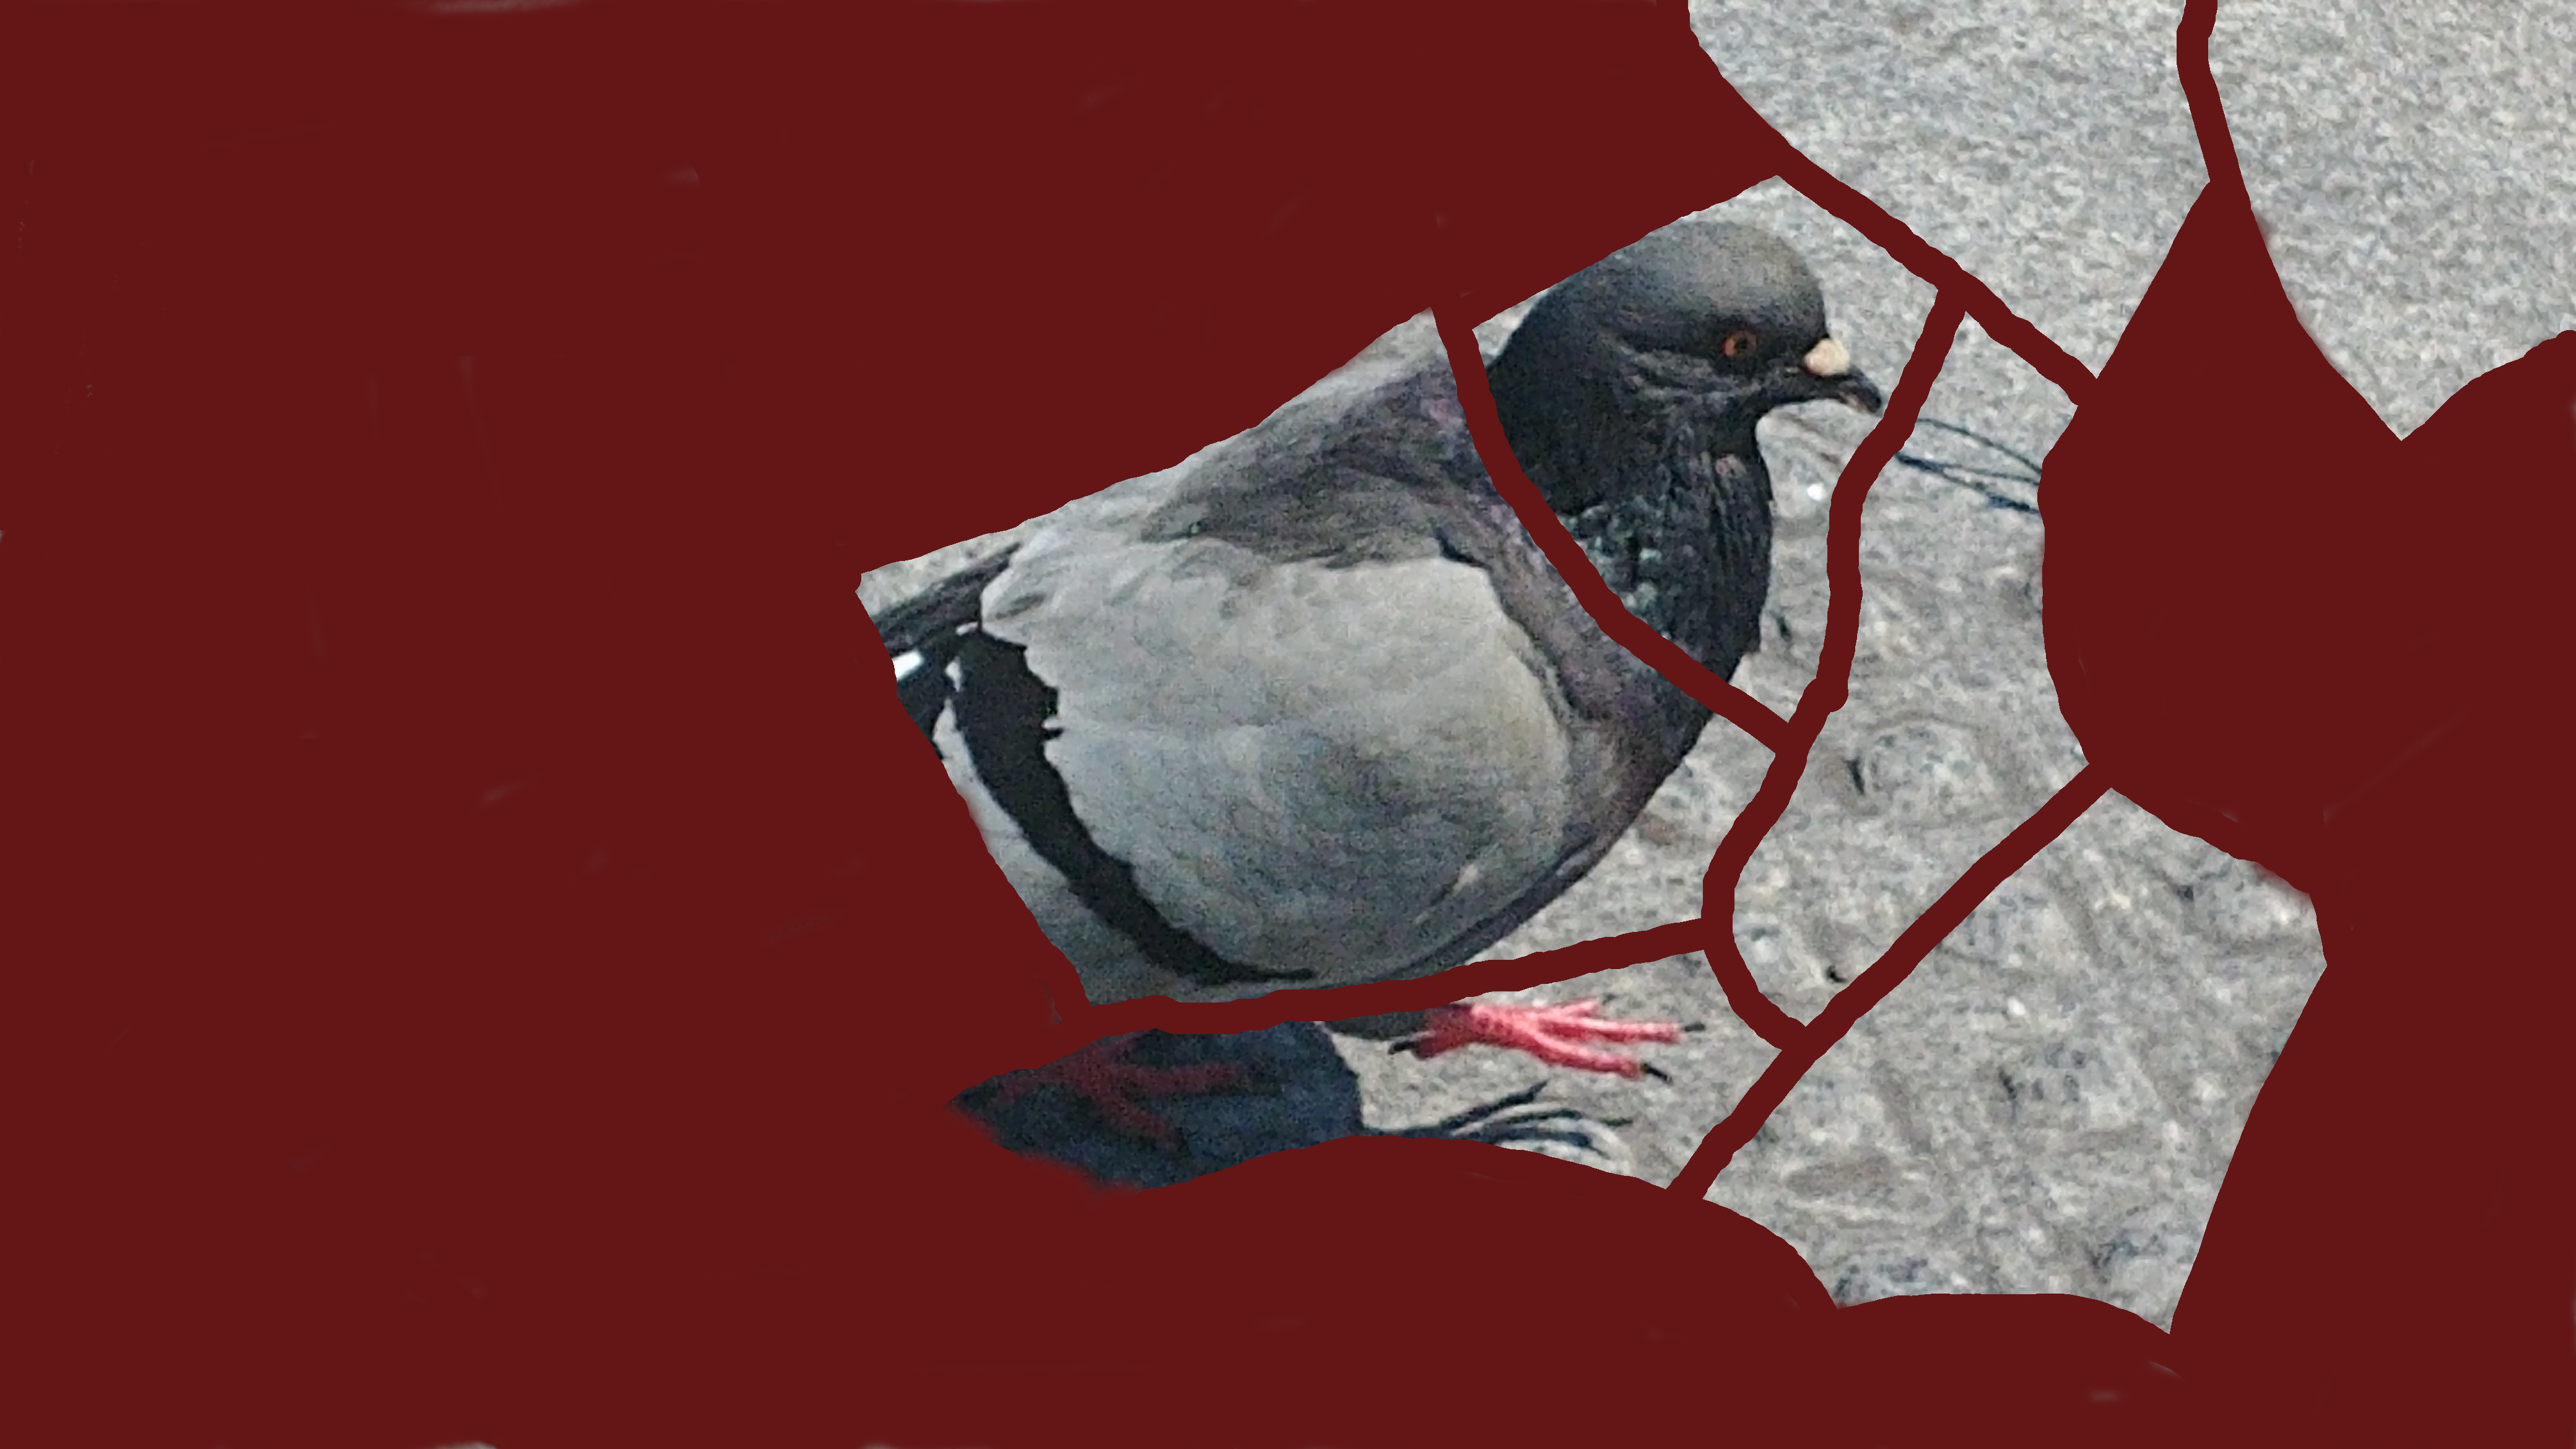
\includegraphics[width=\linewidth]{images/lime/pert3}
        \caption{Perturbation 3}
    \end{subfigure}
    \caption{Greyed-out images forming a new dataset}
    \label{fig:limegrey}
\end{figure}

Using this data it is possible to determine the importance of regions/features of this particular sample. This importance is local and has a meaning only in relation to the sample image from figure~\ref{fig:limepigeon}. 

\subsection{ELI5}
ELI5 (Explain like I am a 5-year old) is a tool, in form of a Python package, used to debug machine learning classifiers and explain their predictions. It supports multiple machine learning frameworks, including scikit-learn. It can be used to explain how the model works both locally for one prediction and globally for the whole model. The output can take several forms just like in LIME case.

For white-box models, ELI5 works as an extension of scikit-learn and it is capable to extract the weights of model's features for different classes. In addition to that it can show the weights that contributed in a particular prediction. It is done by removing particular features and checking how the accuracy of the classifier was altered. On the other hand, for black-box models, this tool integrates a modified version of LIME, supporting more machine learning frameworks, and a permutation importance method, which checks how the model's accuracy decreases when removing one of the features and on this basis determines the importance of the features.

\subsection{YellowBrick}
YellowBrick is another Python package, which is an extension of scikit-learn framework. It is meant to give global interpretation of the analysed model on different levels. It is possible not only to visualize features importances calculated directly by scikit-learn, but also to give a classification report (accuracy, recall, precision, f-measure), plot a confusion matrix, a ROC curve and much more. In addition to all that, YellowBrick comes with a tool for determination of correlation between features in the dataset.

\subsection{Treeinterpreter}
Treeinterpreter is a simple Python package that works with scikit-learn trees and random forest classifiers. It's only usage consists in decomposing the obtained prediction into bias and contributions of different features. The output is given in the form of a numpy array.

\subsection{scikit-learn export\_graphviz}
export\_graphviz is a scikit-learn embedded function that enables the user to visualize a decision tree with all the branches and save it into Graphviz\footnote{a set of tools for diagram creation using graphs.} format, that can be converted into a vector graphic. It is possible also to visualize decision trees composing random forest model in scikit-learn, since the possibility to extract particular decision trees when using this framework. However the interpretability of results for random forest classifier can be hard.

\subsection{dtreeviz}
dtreeviz is a more advanced version of export\_graphviz available in scikit-learn. For every leaf in the tree it can show a histogram indicating the influence of feature's value on class selection. In addition to that, dtreeviz enables the user to show the path of a particular prediction. The result is saved in the form of a svg vector graphic. 

% \begin{figure}[tb]
%     \centering
%     \makebox[\textwidth]{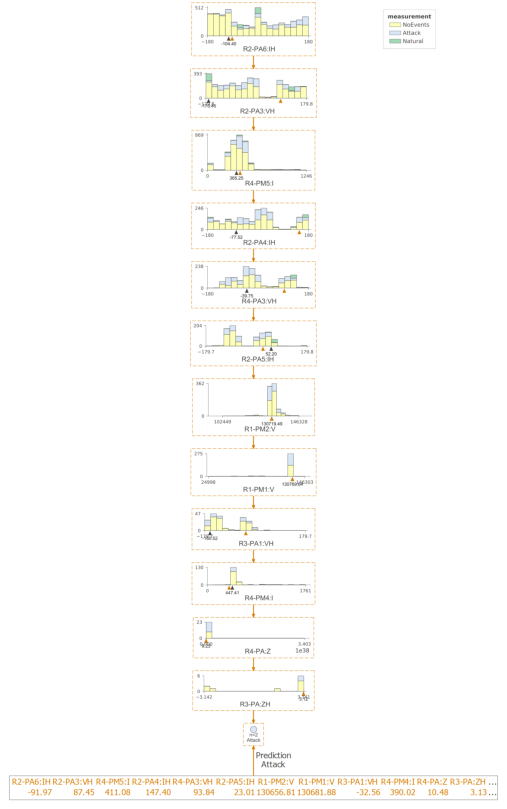
\includegraphics[width=.9\paperwidth, height=.9\textheight]{images/dtreeviz}}
%     \caption{dtreeviz's visualisation of the prediction path for Natural event mispredicted as Attack}
%     \label{fig:dtreeviz}
% \end{figure}



\subsection{Summary}
It can be concluded that ELI5 is the most versatile package compared to others, especially because it enables both global and local interpretations and does not limit its support to scikit-learn, plus it has LIME integrated in it. YellowBrick, on other hand, adds the possibility to analyse from a statistical view the features available in the dataset. Finally comes Treeinterpreter and dtreeviz that are interesting tools when analysing especially Decision Trees. A summary of the most import features of all 5 packages is shown in table \ref{tab:comp}, where 6 comparison metrics where taken into consideration:
\begin{itemize}
    \item global interpretation: capacity of the tool to interpret the whole model,
    \item local interpretation: capacity of the tool to interpret a particular sample from the dataset,
    \item black-box models support: the fact if the tool supports only black-box models (models that can not be simply interpreted),
    \item features' statistical analysis: the fact if the tool supports statistical analysis of features in the dataset, without taking into consideration the model,
    \item works only with scikit-learn,
    \item decision trees graphical visualization.
\end{itemize}

\begin{table}[H]
    \centering
    \caption{Comparison of tools for model analysis} \label{tab:comp}
    \begin{tabular}{lccccc} \toprule
        & LIME & ELI5 & YellowBrick & Treeinterpreter & dtreeviz \\\midrule
        Global interpretation & \xmark & \cmark & \cmark & \xmark & \xmark \\
        Local interpretation & \cmark & \cmark & \xmark & \cmark & \cmark \\
        Black-box models support & \cmark & \cmark & \cmark & \xmark & \xmark \\
        Features' statistical analysis & \xmark & \xmark & \cmark & \xmark & \xmark \\
        Works only with scikit-learn & \cmark & \xmark & \cmark & \cmark & \cmark \\
        Decision Trees graphical visualization & \xmark & \xmark & \xmark & \xmark & \cmark \\
        \bottomrule
    \end{tabular}
\end{table}

\section{Features' importance determination}
%Lime
For the rest of the chapter LIME was chosen to determine the features' importance because of it working with all black-box models available in scikit-learn. The capabilities of LIME were sufficient and that is why ELI5 was not used in his place.

In what follows the Decision Tree classifier will be used because its ease of interpretation. The explication of the algorithm was provided in \ref{sec:rf} as the part of Random Forest classifier algorithm, since the Random Forest is composed of a certain number of Decision Trees.

Because in this case the explanations of single samples are not really interesting, an attempt to generalize the results was made: Lime explainer was run on 100 false predictions of a chosen class made using Decision Tree classifier. The results are concatenated together. For all the duplicates of features, the mean importance is calculated and only one entry is kept along with this calculated mean value. In other words:

\begin{python}
import pandas as pd
import numpy as np
from lime.lime_tabular import LimeTabularExplainer

# explainer initialization with training data
explainer = LimeTabularExplainer(X, training_labels = y, feature_names = features, class_names = labels)

# Xall = all samples, yall = all true classes corresponding to samples (not used in training)
boole = (yall != clf.predict(Xall)) # all false predicitions
faulty = boole & (yall == 0) # false predicitions of true class equal 0 (NoEvents)
X_test = Xall[faulty] # all false predicition samples
y_test = yall[faulty] # all false predicition true classes
lst = [] # initialization of a list
for idx in range(0, 100): # create explanation for 100 first samples
    exp = explainer.explain_instance(X_test[idx], clf.predict_proba, num_features=128, labels=[0, 1, 2])
    lst.append(exp.as_list(label=0))
# transform to dataframe
lst = np.array(lst)
clst = np.concatenate(lst, axis=0)
dtfr = pd.DataFrame(clst, columns=['feature', 'importance'])
dtfr["importance"] = pd.to_numeric(dtfr["importance"])
# group by feature then sort
dtfr = dtfr.groupby(['feature']).mean()
res = dtfr.sort_values(by="importance")
\end{python}

The results, reduced to 5 most important features for NoEvents, Attack, Natural and all samples, are shown respectively in tables \ref{tab:5best:noev}, \ref{tab:5best:attack} and \ref{tab:5best:natural}.

\begin{table}[H]
    \centering
    \caption{5 most important features for NoEvents samples} \label{tab:5best:noev}
    \begin{tabular}{lr}\toprule
        feature  &importance\\\midrule            
        R4-PA5:IH > 115.38                  & 0.008534\\
        R3-PM2:V <= 128425.29               & 0.007998\\
        128762.21 < R2-PM1:V <= 129859.49   & 0.007776\\
        0.00 < R1-PA12:IH <= 32.04          & 0.007514\\
        R3-PM5:I <= 330.70                  & 0.005762\\
        ...                                 & ... \\\bottomrule
    \end{tabular}
\end{table}

\begin{table}[H]
    \centering
    \caption{5 most important features for Attack samples} \label{tab:5best:attack}
    \begin{tabular}{lr}\toprule
        feature                   & importance \\\midrule
        R3:S > 0.00                    & 0.010717  \\
        R2-PA7:VH <= -101.20           & 0.014018   \\
        R2-PM1:V > 130872.03           & 0.009242 \\
        R3-PA7:VH <= -101.22           & 0.008676 \\
        R3-PA2:VH <= -93.75            & 0.008307 \\
        ...                            & ... \\\bottomrule
    \end{tabular}
\end{table}

\begin{table}[H]
    \centering
    \caption{5 most important features for Natural samples} \label{tab:5best:natural}
    \begin{tabular}{lr}\toprule
        feature                & importance   \\\midrule    
        R2:F > 60.00           &  0.005168 \\
        R3:F > 60.00           &  0.004873 \\
        R2-PA5:IH > 63.30      &  0.004103 \\
        R2-PM7:V > 130857.40   &  0.003693 \\
        R1-PA1:VH > 71.28     &   0.003518 \\
        ...                    &       ...    \\\bottomrule
    \end{tabular}
\end{table}

% \begin{table}[H]
%     \centering
%     \caption{5 most important features for all samples} \label{tab:5best:all}
%     \begin{tabular}{lr}\toprule
%         feature                   &    importance   \\ \midrule                            
%         R2-PM1:V > 130872.03     &      0.009070   \\
%         R3-PM2:V > 130431.15      &     0.008501 \\
%         R4-PA1:VH > 71.50         &     0.007481 \\
%         R3-PA4:IH > 102.49        &     0.005723 \\
%         R2-PA3:VH <= -75.28      &      0.005588 \\
%         ...                       &          ... \\\bottomrule
%     \end{tabular}
% \end{table}

It can be observed that the five most important features among false predictions for each class are different. This implies creating a correction model for every important feature among all classes. The exact procedure is described in the next chapter.

In this chapter different result interpreters were presented in details. Among them, Lime have been chosen to create an algorithm for features importance determination. The most important features will be used in next chapter to correct the obtained predictions. 
\chapter{Model enhancement}
After having chosen the appropriate machine learning algorithms and found a way to determine the most important features in the classification problem, this chapter is an attempt to create a model able to enhance the results obtained by the basic classification. Three different approaches are presented. First of all, the most important features values were altered and the effect of this modification is examined. Second, a formula for calculating the distance between different samples is established then a way to use that information. Finally, the Hidden Markov Model were used in order to determine the likehood of prediction of a particular class and this data was used to modify the machine learning algorithm. 

\section{Features values modification}
The first proposed solution considers changing the values of most important features in the dataset after the training process. In other words the training process occurs normally, then the importances are determined and a correction function is created (figure \ref{fig:train}). This correction function will act then on the samples introduced to the model in order to change the features values and obtain better predictions (figure \ref{fig:predict}). 

\begin{figure}[H]
    \centering
    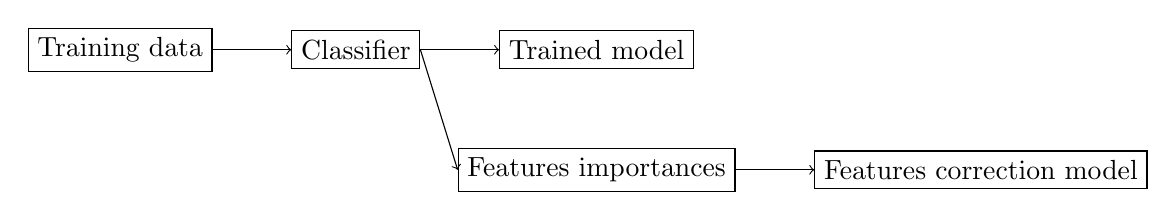
\begin{tikzpicture}
        \node[rectangle, draw=black] (main) {Training data};
        \node[rectangle, draw=black] (DecisionTree) [right=of main] {Classifier};
        \node[rectangle, draw=black] (out1) [right=of DecisionTree] {Trained model};
        \node[rectangle, draw=black] (out2) [below=of out1] {Features importances};
        \node[rectangle, draw=black] (feat) [right=of out2] {Features correction model};
   
        \draw[->] (main.east) -- (DecisionTree.west);
        \draw[->] (DecisionTree.east) -- (out1.west);
        \draw[->] (DecisionTree.east) -- (out2.west); 
        \draw[->] (out2.east) -- (feat.west);
    \end{tikzpicture}
    \caption{Training process illustration} \label{fig:train}
\end{figure}

\begin{figure}[H]
    \centering
    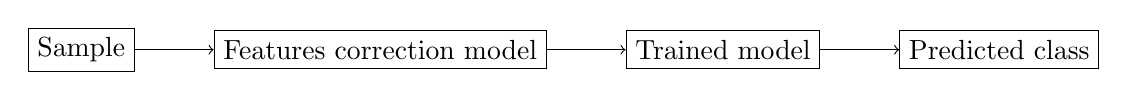
\begin{tikzpicture}
        \node[rectangle, draw=black] (main) {Sample};
        \node[rectangle, draw=black] (correl) [right=of main] {Features correction model};
        \node[rectangle, draw=black] (model) [right=of correl] {Trained model};
        \node[rectangle, draw=black](out) [right=of model] {Predicted class};

        \draw[->] (main.east) -- (correl.west);
        \draw[->] (correl.east) -- (model.west);
        \draw[->] (model.east) -- (out.west);
    \end{tikzpicture}
    \caption{Prediction illustration} \label{fig:predict}
\end{figure}

First of all the correction function was defined as the modification function of the feature values for the predicted samples. This modification consists in shifting the feature value so the feature value would not meet the condition to make a false prediction from tables \ref{tab:5best_dt}-\ref{tab:5best_mlp}. This function code in Python is as follows:  
\begin{python}
def modify(feat, val):
    X[feat] = X[feat].apply(lambda x: x + val)
\end{python}
where \textit{X} is a pandas DataFrame object containing all the samples to predict.

Second, the five most important features are taken from tables \ref{tab:5best_dt}-\ref{tab:5best_mlp} and the values of features from the samples to predict are altered using the previous function. If a feature is duplicated only the value of the first occurrence is taken into account. The following code shows this operation for Decision Tree classifier:

\begin{python}
modify("R4-PA5:IH", -115.38)
modify("R3-PM2:V", 128525.29)
modify("R2-PM1:V", 2000)
modify("R1-PA12:IH", 32.04)
modify("R3-PM5:I", 330.7)
modify("R3:S", 0)
modify("R2-PA7:VH", 101.20)
modify("R2-PM1:V", -1300872.03)
modify("R3-PA7:VH", 101.22)
modify("R3-PA2:VH", 93.75)    
modify("R2:F", -60)
modify("R3:F", -60)
modify("R2-PA5:IH",- 63.30)
modify("R2-PM7:V", -130857.40) 
\end{python}

The samples modified this way are then used for the predictions. In order to check the success of this method, the classification\_report method from scikit-learn was used. The results before and after modifying the samples are displayed for Decision Tree, Random Forest and MLP classifiers respectively in tables \ref{tab:fm_dt}, \ref{tab:fm_rf} and \ref{tab:fm_mlp}.

\begin{table}[H]
    \centering
    \footnotesize
    \caption{Features modification results for Decision Tree classifier} \label{tab:fm_dt}
    \begin{subtable}[t]{.5\linewidth}
        \centering
        \caption{Before features modification} 
        \begin{tabular}{rcccc}\toprule
            & precision    &recall & f1-score  & support \\\midrule
                NoEvents  &   $  0.72 $  &  $ 0.76 $  &  $ 0.74 $  & $ 51797 $\\
                  Attack   &  $  0.27 $   & $ 0.26 $  &  $ 0.26 $  & $ 17382 $\\
                 Natural   &  $  0.19 $   & $ 0.08 $  &  $ 0.12 $  & $  4232 $\\
                accuracy   &            &          &  $0.60$  &   $73411$ \\
               macro avg   &  $  0.39 $   & $ 0.37 $  &  $ 0.37 $  & $ 73411 $\\
            weighted avg   &  $  0.58 $  &  $ 0.60 $  &  $ 0.59 $ &  $ 73411 $\\\bottomrule
        \end{tabular}
    \end{subtable}%
    \begin{subtable}[t]{.5\linewidth}
        \centering
        \caption{After features modification}
        \begin{tabular}{rcccc}\toprule
            &precision   & recall & f1-score &  support  \\\midrule
    
            NoEvents   &    0.71   &   0.83  &    0.77   &  51797 \\
              Attack    &   0.26   &   0.17  &    0.21   &  17382 \\
             Natural   &    0.10   &   0.03   &   0.05  &    4232 \\
        
            accuracy    &          &          &   0.63   &  73411 \\
           macro avg    &   0.36   &   0.34   &   0.34   &  73411 \\
        weighted avg     &  0.57   &   0.63   &   0.59   &  73411    \\     \bottomrule   
        \end{tabular}
    \end{subtable}
\end{table}

\begin{table}[H]
    \centering
    \footnotesize
    \caption{Features modification results for Random Forest classifier} \label{tab:fm_rf}
    \begin{subtable}[t]{.5\linewidth}
        \centering
        \caption{Before features modification} 
        \begin{tabular}{rcccc}\toprule
            & precision    &recall & f1-score  & support \\\midrule
            NoEvents   &    0.72  &    0.87 &     0.78 &  51797 \\
            Attack     &  0.29    &  0.16   &   0.21   &  17382 \\
           Natural     &  0.25    &  0.05   &   0.08   &   4232 \\
          accuracy     &          &         &   0.65   &  73411 \\
         macro avg     &  0.42    &  0.36   &   0.36   &  73411 \\
      weighted avg     &  0.59    &  0.65   &   0.61   &  73411 \\ \bottomrule
        \end{tabular}
    \end{subtable}%
    \begin{subtable}[t]{.5\linewidth}
        \centering
        \caption{After features modification}
        \begin{tabular}{rcccc}\toprule
            &precision   & recall & f1-score &  support  \\\midrule
            NoEvents  &     0.71 &     0.89 &     0.79 &  51797\\
            Attack    &   0.28   &   0.13   &   0.18   &  17382\\
           Natural    &   0.26   &   0.05   &   0.08   &   4232\\
          accuracy    &          &          &   0.66   &  73411\\
         macro avg    &   0.42   &   0.36   &   0.35   &  73411\\
      weighted avg    &   0.58   &   0.66   &   0.61   &  73411\\     \bottomrule   
        \end{tabular}
    \end{subtable}
\end{table}

\begin{table}[H]
    \centering
    \footnotesize
    \caption{Features modification results for MLP classifier} \label{tab:fm_mlp}
    \begin{subtable}[t]{.5\linewidth}
        \centering
        \caption{Before features modification} 
        \begin{tabular}{rcccc}\toprule
            & precision    &recall & f1-score  & support \\\midrule
            NoEvents   &    0.71 &     0.99 &     0.83&    51797\\
            Attack     &  0.57   &   0.05   &   0.09  &   17382\\
           Natural     &  0.00   &   0.00   &   0.00  &    4232\\    
          accuracy     &         &          &   0.71  &   73411\\
         macro avg     &  0.43   &   0.35   &   0.30  &   73411\\
      weighted avg     &  0.64   &   0.71   &   0.60  &   73411\\ \bottomrule
        \end{tabular}
    \end{subtable}%
    \begin{subtable}[t]{.5\linewidth}
        \centering
        \caption{After features modification}
        \begin{tabular}{rcccc}\toprule
            &precision   & recall & f1-score &  support  \\\midrule
            NoEvents   &    0.74  &    0.07 &     0.12 &  51797\\
            Attack     &  0.24    &  0.93   &   0.38   &  17382\\
           Natural     &  0.00    &  0.00   &   0.00   &   4232\\   
          accuracy     &          &         &   0.27   &  73411\\
         macro avg     &  0.33    &  0.33   &   0.17   &  73411\\
      weighted avg     &  0.58    &  0.27   &   0.17   &  73411\\    \bottomrule   
        \end{tabular}
    \end{subtable}
\end{table}

The accuracy of the model has slightly increased for both Decision Tree and Random Forest classifiers, and significally decreased for MLP classifier. Moreover, for Decision Tree classifier, a significant decrease of other metrics for Natural class is observed, for Random Forest some slight increases and decreases of metrics are observed, depending on the class. The most important difference is observed for MLP classifier, where the recall value for NoEvents class passed from $0.99$ to $0.07$, and in parallel, for Attack class from $0.05$ to $0.93$.

It may be concluded that this method succeeded to enhance the results for Decision Tree and Random Forest classifiers, but failed with MLP. It is clear that the model, after modifying the features, tends to predict NoEvents class for the first two classifiers, but Attack class for MLP.  

\section{Distance between features}
The second proposed solution considers using a transformation routine, which, reduces the number of features to the 15 most important from tables \ref{tab:5best_dt}-\ref{tab:5best_mlp} and adds another feature that represents the closest class to the treated sample. The prediction steps were illustrated on figure \ref{fig:distill}.

\begin{figure}[H]
    \centering
    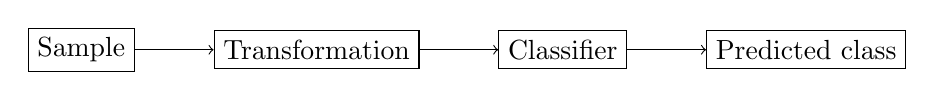
\begin{tikzpicture}
        \node[rectangle, draw=black](sample) {Sample};
        \node[rectangle, draw=black](trans) [right=of sample] {Transformation};
        \node[rectangle, draw=black](class) [right=of trans] {Classifier};
        \node[rectangle, draw=black](out) [right=of class] {Predicted class};

        \draw[->] (sample.east) -- (trans.west);
        \draw[->] (trans.east) -- (class.west);
        \draw[->] (class.east) -- (out.west);
    \end{tikzpicture}
    \caption{Distance algorithm illustration}
    \label{fig:distill}
\end{figure}

The transformation routine on other hand takes the form of a python class and is composed of 4 methods:
\begin{enumerate}
    \item \textbf{distance(X1, X2)}: returns the distance between two samples X1 and X2. It is calculated as the sum of differences between features,
    \item \textbf{important(X)}: returns the samples with only 15 most important features. The input must be a pandas DataFrame or Series. The choice of features to keep is made by hand directly in the method, without the possibility to change them afterwards,
    \item \textbf{fit(X,y)}: determines the reference class sample for each class by calculating the mean value of each feature among all samples corresponding to the treated class. It is called only during data fitting to the classifier,
    \item \textbf{transform(X)}: determines the class with the smallest distance to the sample, based on reference samples determined by fit(X,y) method. The obtained values are then added as a new feature to the samples X and returned afterwards by the method.
\end{enumerate}

This routine has been coupled with the 3 chosen classifiers using \textbf{pipeline} class in scikit-learn, which construct acts like a classifier (it has fit and predict methods). 

The success rate of this method was verified, once more, using classification\_report method from scikit-learn. The result and after using the described method are shown for Decision Tree, Random Forest and MLP classifiers respectively in tables \ref{tab:dist_dt}, \ref{tab:dist_rf} and \ref{tab:dist_mlp}.

\begin{table}[H]
    \centering \footnotesize
    \caption{Distance routine results for Decision Tree classifier}  \label{tab:dist_dt}
    \begin{subtable}[t]{.5\linewidth}
        \centering
        \caption{Before using the distance routine} 
        \begin{tabular}{rcccc}\toprule
            & precision    &recall & f1-score  & support \\\midrule
                NoEvents  &   $  0.72 $  &  $ 0.76 $  &  $ 0.74 $  & $ 51797 $\\
                  Attack   &  $  0.27 $   & $ 0.26 $  &  $ 0.26 $  & $ 17382 $\\
                 Natural   &  $  0.19 $   & $ 0.08 $  &  $ 0.12 $  & $  4232 $\\
                accuracy   &            &          &  $0.60$  &   $73411$ \\
               macro avg   &  $  0.39 $   & $ 0.37 $  &  $ 0.37 $  & $ 73411 $\\
            weighted avg   &  $  0.58 $  &  $ 0.60 $  &  $ 0.59 $ &  $ 73411 $\\\bottomrule
        \end{tabular}
    \end{subtable}%
    \begin{subtable}[t]{.5\linewidth}
        \centering
        \caption{After using the distance routine} 
        \begin{tabular}{rcccc}\toprule
         &   precision    &recall & f1-score &  support  \\\midrule
    
            NoEvents    &   0.72   &   0.79   &   0.75  &   51797 \\
              Attack    &   0.28   &   0.23   &   0.25  &   17382 \\
             Natural   &    0.19   &   0.08   &   0.11  &    4232 \\
        
            accuracy    &           &         &   0.62   &  73411 \\
           macro avg    &   0.40    &  0.37   &   0.37  &   73411 \\
        weighted avg   &   0.58   &   0.62   &   0.60   &  73411   \\  \bottomrule
        \end{tabular}
    \end{subtable}
\end{table}

\begin{table}[H]
    \centering \footnotesize
    \caption{Distance routine results for Random Forest classifier}  \label{tab:dist_rf}
    \begin{subtable}[t]{.5\linewidth}
        \centering
        \caption{Before using the distance routine} 
        \begin{tabular}{rcccc}\toprule
            & precision    &recall & f1-score  & support \\\midrule
            NoEvents   &    0.72  &    0.87 &     0.78 &  51797 \\
            Attack     &  0.29    &  0.16   &   0.21   &  17382 \\
           Natural     &  0.25    &  0.05   &   0.08   &   4232 \\
          accuracy     &          &         &   0.65   &  73411 \\
         macro avg     &  0.42    &  0.36   &   0.36   &  73411 \\
      weighted avg     &  0.59    &  0.65   &   0.61   &  73411 \\ \bottomrule
        \end{tabular}
    \end{subtable}%
    \begin{subtable}[t]{.5\linewidth}
        \centering
        \caption{After using the distance routine} 
        \begin{tabular}{rcccc}\toprule
         &   precision    &recall & f1-score &  support  \\\midrule
    
        NoEvents   &    0.71 &     0.83 &     0.77 &   51797\\
         Attack    &   0.27  &    0.19  &    0.22  &   17382\\
        Natural    &   0.18  &    0.05  &    0.07  &    4232\\
       accuracy    &         &          &    0.63  &   73411\\
      macro avg    &   0.39  &    0.36  &    0.36  &   73411\\
   weighted avg    &   0.58  &    0.63  &    0.60  &   73411\\  \bottomrule
        \end{tabular}
    \end{subtable}
\end{table}

\begin{table}[H]
    \centering \footnotesize
    \caption{Distance routine results for MLP classifier}  \label{tab:dist_mlp}
    \begin{subtable}[t]{.5\linewidth}
        \centering
        \caption{Before using the distance routine} 
        \begin{tabular}{rcccc}\toprule
            & precision    &recall & f1-score  & support \\\midrule
            NoEvents   &    0.71 &     0.99 &     0.83&    51797\\
            Attack     &  0.57   &   0.05   &   0.09  &   17382\\
           Natural     &  0.00   &   0.00   &   0.00  &    4232\\    
          accuracy     &         &          &   0.71  &   73411\\
         macro avg     &  0.43   &   0.35   &   0.30  &   73411\\
      weighted avg     &  0.64   &   0.71   &   0.60  &   73411\\ \bottomrule
        \end{tabular}
    \end{subtable}%
    \begin{subtable}[t]{.5\linewidth}
        \centering
        \caption{After using the distance routine} 
        \begin{tabular}{rcccc}\toprule
         &   precision    &recall & f1-score &  support  \\\midrule
    
         NoEvents  &     0.70 &     0.98 &     0.82 &  51797\\
         Attack    &   0.18   &   0.01   &   0.02   &  17382\\
        Natural    &   0.00   &   0.00   &   0.00   &   4232\\
       accuracy    &          &          &   0.69   &  73411\\
      macro avg    &   0.29   &   0.33   &   0.28   &  73411\\
   weighted avg    &   0.54   &   0.69   &   0.58   &  73411\\  \bottomrule
        \end{tabular}
    \end{subtable}
\end{table}

The tables \ref{tab:dist_dt}-\ref{tab:dist_mlp} show an increase of accuracy by 0.02 in the Decision Tree classifier case, but a decrease by also 0.02 in the Random Forest and MLP classifiers case. For Decision Tree classifier, the other metrics shows a slight increase, except recall and f-measure for Attack class, however this decrease was not significant. On other hand for the two remaining classifiers a decrease in values of almost all the metrics is observed.

It can be concluded that this method does work only using Decision Tree classifier and gives results better than the features' modification method. For Random Forest and MLP classifiers this method fails to enhance the predictions.

\section{Hidden Markov Model}
The last proposed solution consists in determining the probabilities of occurrence of different classes using so called Hidden Markov Model. The obtained probabilities are then used to modify the split condition in the decision tree classifier. 

The Hidden Markov Model is a probabilistic model for generating observable data in a random way by a sequence of internal hidden states, which can not be observed directly. The transitions between those hidden states have the form of a Markov chain \cite{noauthor_tutorial_nodate}. The Markov chain, on other hand, is a chain of interconnected states, where each state's probability depends only of the probability of predecessing state, without taking into consideration what happened before \cite{amit_introduction_2019}.

In the studied example, the observable data are the features values available in the samples and the states are represented by the 3 classes NoEvents, Attack and Normal. The Hidden Markov Model was used to determine the stationary distribution of the states (invariable in time probability distribution in the Markov chain).

It exists a Python package that implements the Hidden Markov Models and it is compatible with scikit-learn, it's name is \textbf{hmmlearn} \cite{noauthor_hmmlearn_2020}. It can be used just like any other scikit-learn classifiers, especially that it offers methods like fit(), predict(), predict\_proba(), etc...

Using \textbf{hmmlearn} the stationary distribution was determined in 4 lines of code:
\begin{python}
from hmmlearn.hmm import GaussianHMM 
clf2 = GaussianHMM(n_components = 3) # 3 states
clf2.fit(X)
coefs = clf2.get_stationary_distribution()
\end{python}
The Gaussian HMM was used because the observations (features) are continuous. It was initialized by a number of components equal to 3 because of 3 states - NoEvents, Attack and Natural.

The stationary distribution obtained this way was then used to set the class\_weight parameter in DecisionTreeClassifier in scikit-learn, as shown in the listing below.

\begin{python}
ctest = DecisionTreeClassifier(class_weight = {0: coefs[0], 1:coefs[1], 2:coefs[2]})  
\end{python}

For Random Forest classifier the same parameter exists and was used to produce results. However, for MLP classifier a similar parameter does not exist and using the determined coefficients would require deeper modifications of the neural network.

The results for Decision Tree and Random Forest classifiers are presented in tables \ref{tab:hmm_dt} and \ref{tab:hmm_rf}.

\begin{table}[H]
    \centering \footnotesize
    \caption{Hidden Markov Model manipulation results for Decision Tree classifier}  \label{tab:hmm_dt}
    \begin{subtable}[t]{.5\linewidth}
        \centering
        \caption{Before using HMM} 
        \begin{tabular}{rcccc}\toprule
            & precision    &recall & f1-score  & support \\\midrule
                NoEvents  &   $  0.72 $  &  $ 0.76 $  &  $ 0.74 $  & $ 51797 $\\
                  Attack   &  $  0.27 $   & $ 0.26 $  &  $ 0.26 $  & $ 17382 $\\
                 Natural   &  $  0.19 $   & $ 0.08 $  &  $ 0.12 $  & $  4232 $\\
                accuracy   &            &          &  $0.60$  &   $73411$ \\
               macro avg   &  $  0.39 $   & $ 0.37 $  &  $ 0.37 $  & $ 73411 $\\
            weighted avg   &  $  0.58 $  &  $ 0.60 $  &  $ 0.59 $ &  $ 73411 $\\\bottomrule
        \end{tabular}
    \end{subtable}%
    \begin{subtable}[t]{.5\linewidth}
        \centering
        \caption{After using HMM}
        \begin{tabular}{rcccc}\toprule
        & precision &   recall & f1-score  & support \\\midrule

            NoEvents    &   0.71    &  0.75  &    0.73     &51797\\
            Attack     &  0.27    &  0.26  &    0.26 &   17382\\
            Natural    &   0.16  &    0.06    &  0.09  &    4232\\
        
            accuracy     &          &         &   0.60   &  73411\\
        macro avg     &  0.38    &  0.36   &   0.36  &   73411\\
        weighted avg    &   0.58    &  0.60   &   0.59  &   73411   \\ \bottomrule   
        \end{tabular}
    \end{subtable}
\end{table}

\begin{table}[H]
    \centering \footnotesize
    \caption{Hidden Markov Model manipulation results for Random Forest classifier}  \label{tab:hmm_rf}
    \begin{subtable}[t]{.5\linewidth}
        \centering
        \caption{Before using HMM} 
        \begin{tabular}{rcccc}\toprule
            & precision    &recall & f1-score  & support \\\midrule
            NoEvents   &    0.72  &    0.87 &     0.78 &  51797 \\
            Attack     &  0.29    &  0.16   &   0.21   &  17382 \\
           Natural     &  0.25    &  0.05   &   0.08   &   4232 \\
          accuracy     &          &         &   0.65   &  73411 \\
         macro avg     &  0.42    &  0.36   &   0.36   &  73411 \\
      weighted avg     &  0.59    &  0.65   &   0.61   &  73411 \\ \bottomrule
        \end{tabular}
    \end{subtable}%
    \begin{subtable}[t]{.5\linewidth}
        \centering
        \caption{After using HMM}
        \begin{tabular}{rcccc}\toprule
        & precision &   recall & f1-score  & support \\\midrule
        NoEvents   &    0.72 &     0.85  &    0.78 &  51797\\
        Attack     &  0.30   &   0.19    &  0.24   &  17382\\
       Natural     &  0.25   &   0.05    &  0.09   &   4232\\
      accuracy     &         &           &  0.65   &  73411\\
     macro avg     &  0.42   &   0.37    &  0.37   &  73411\\
  weighted avg     &  0.59   &   0.65    &  0.61   &  73411\\ \bottomrule   
        \end{tabular}
    \end{subtable}
\end{table}

The tables \ref{tab:hmm_dt} and \ref{tab:hmm_rf} show that the accuracy did not change after using the probabilities obtained from Hidden Markov Model. Looking more in details, it can be observed a general small decrease of the majority of the other metrics in the Decision Tree classifier case, but, in Random Forest classifier case, a slight increase in metrics value in relation to the Attack class and a small decrease of recall for NoEvents.

It may be concluded that this method does not work with the given dataset, however the results obtained by the Random Forest classifier are better than those provided by Decision Tree classifier. The possible cause of the failure of this method may be the fact that the samples in the dataset does not include any information about their order in time. If the dataset contained information about the time of the event, the results, probably, would be more significant. \\

In this chapter, three methods for results' enhancement were presented. The results vary depending on the used machine learning technique. For Decision Tree classifier, the best method for enhancing the results was the second, using the distance between features. For Random Forest classifier, the best method was the first, modifying the values of features. Finally, for MLP classifier, both two tested methods failed, but the second did not decrease the metrics that drastically as the first method.
\chapter{Conclusions}

The aim of this thesis was to develop a hybrid neural network capable of differentiating between three states of a cyber physical system - normal behaviour, a fault or an attack. To facilitate the work and focus on computer science topics, ready datasets for a power system was taken and analysed in chapter 2. 

Three different methods were presented to achieve the initial goal - modification of values of features, method using distances between samples and a method using Hidden Markov Model. They were tested on three different machine learning classifiers - Decision Tree, Random Forest and Multilayer Perceptron. 

For Decision Tree classifier the most efficient enhancement method was using the proposed method that works on distances between samples. For Random Forest classifier, the most effective method was modifying the values of features. And for Multilayer Perceptron classifier all the proposed methods failed.

Hidden Markov Model method gave the smallest impact on the tested classifiers. This can be explained by the time independence of the used dataset, especially that this method relies on order of samples.

A possible better solution for the posed problem may be using a physical model of the power system that could estimate on its own some features and combining it with a machine learning technique. There exist some python toolkits created to model a power system like PyPSA \cite{brown_pypsapypsa_2020} or pandapower \cite{noauthor_pandapower_nodate}, but they are complex and require specific advanced technical skills.

This thesis in addition to all that, provides some other important conclusions. First, the different machine learning toolkits do not work always the same way and the results may differ from one toolkit to another, like in this case and the differences in results between Weka and scikit-learn. Second, in order to the results from a work to be reproductible, all the details concerning the used parameters and the version of the software must be provided, in other case it may be hard to get the same result. Finally, it exists plenty of tools for machine learning classifiers evaluation and each toolkit provides its own interpretation of results.

This work may be continued by implementing the power system using one of the mentioned toolkits in order to try to further enhance the results. In addition to that, instead of using scikit-learn, Keras \cite{noauthor_keras_nodate} or PyTorch \cite{noauthor_pytorch_nodate} packages may be used in order to create a complex neural network and possibly get better results.   

%\appendix
\bibliography{main}
\bibliographystyle{ieeetr}

\end{document}

